\documentclass[1p]{elsarticle_modified}
%\bibliographystyle{elsarticle-num}

%\usepackage[colorlinks]{hyperref}
%\usepackage{abbrmath_seonhwa} %\Abb, \Ascr, \Acal ,\Abf, \Afrak
\usepackage{amsfonts}
\usepackage{amssymb}
\usepackage{amsmath}
\usepackage{amsthm}
\usepackage{scalefnt}
\usepackage{amsbsy}
\usepackage{kotex}
\usepackage{caption}
\usepackage{subfig}
\usepackage{color}
\usepackage{graphicx}
\usepackage{xcolor} %% white, black, red, green, blue, cyan, magenta, yellow
\usepackage{float}
\usepackage{setspace}
\usepackage{hyperref}

\usepackage{tikz}
\usetikzlibrary{arrows}

\usepackage{multirow}
\usepackage{array} % fixed length table
\usepackage{hhline}

%%%%%%%%%%%%%%%%%%%%%
\makeatletter
\renewcommand*\env@matrix[1][\arraystretch]{%
	\edef\arraystretch{#1}%
	\hskip -\arraycolsep
	\let\@ifnextchar\new@ifnextchar
	\array{*\c@MaxMatrixCols c}}
\makeatother %https://tex.stackexchange.com/questions/14071/how-can-i-increase-the-line-spacing-in-a-matrix
%%%%%%%%%%%%%%%

\usepackage[normalem]{ulem}

\newcommand{\msout}[1]{\ifmmode\text{\sout{\ensuremath{#1}}}\else\sout{#1}\fi}
%SOURCE: \msout is \stkout macro in https://tex.stackexchange.com/questions/20609/strikeout-in-math-mode

\newcommand{\cancel}[1]{
	\ifmmode
	{\color{red}\msout{#1}}
	\else
	{\color{red}\sout{#1}}
	\fi
}

\newcommand{\add}[1]{
	{\color{blue}\uwave{#1}}
}

\newcommand{\replace}[2]{
	\ifmmode
	{\color{red}\msout{#1}}{\color{blue}\uwave{#2}}
	\else
	{\color{red}\sout{#1}}{\color{blue}\uwave{#2}}
	\fi
}

\newcommand{\Sol}{\mathcal{S}} %segment
\newcommand{\D}{D} %diagram
\newcommand{\A}{\mathcal{A}} %arc


%%%%%%%%%%%%%%%%%%%%%%%%%%%%%5 test

\def\sl{\operatorname{\textup{SL}}(2,\Cbb)}
\def\psl{\operatorname{\textup{PSL}}(2,\Cbb)}
\def\quan{\mkern 1mu \triangleright \mkern 1mu}

\theoremstyle{definition}
\newtheorem{thm}{Theorem}[section]
\newtheorem{prop}[thm]{Proposition}
\newtheorem{lem}[thm]{Lemma}
\newtheorem{ques}[thm]{Question}
\newtheorem{cor}[thm]{Corollary}
\newtheorem{defn}[thm]{Definition}
\newtheorem{exam}[thm]{Example}
\newtheorem{rmk}[thm]{Remark}
\newtheorem{alg}[thm]{Algorithm}

\newcommand{\I}{\sqrt{-1}}
\begin{document}

%\begin{frontmatter}
%
%\title{Boundary parabolic representations of knots up to 8 crossings}
%
%%% Group authors per affiliation:
%\author{Yunhi Cho} 
%\address{Department of Mathematics, University of Seoul, Seoul, Korea}
%\ead{yhcho@uos.ac.kr}
%
%
%\author{Seonhwa Kim} %\fnref{s_kim}}
%\address{Center for Geometry and Physics, Institute for Basic Science, Pohang, 37673, Korea}
%\ead{ryeona17@ibs.re.kr}
%
%\author{Hyuk Kim}
%\address{Department of Mathematical Sciences, Seoul National University, Seoul 08826, Korea}
%\ead{hyukkim@snu.ac.kr}
%
%\author{Seokbeom Yoon}
%\address{Department of Mathematical Sciences, Seoul National University, Seoul, 08826,  Korea}
%\ead{sbyoon15@snu.ac.kr}
%
%\begin{abstract}
%We find all boundary parabolic representation of knots up to 8 crossings.
%
%\end{abstract}
%\begin{keyword}
%    \MSC[2010] 57M25 
%\end{keyword}
%
%\end{frontmatter}

%\linenumbers
%\tableofcontents
%
\newcommand\colored[1]{\textcolor{white}{\rule[-0.35ex]{0.8em}{1.4ex}}\kern-0.8em\color{red} #1}%
%\newcommand\colored[1]{\textcolor{white}{ #1}\kern-2.17ex	\textcolor{white}{ #1}\kern-1.81ex	\textcolor{white}{ #1}\kern-2.15ex\color{red}#1	}

{\Large $\underline{12a_{0567}~(K12a_{0567})}$}

\setlength{\tabcolsep}{10pt}
\renewcommand{\arraystretch}{1.6}
\vspace{1cm}\begin{tabular}{m{100pt}>{\centering\arraybackslash}m{274pt}}
\multirow{5}{120pt}{
	\centering
	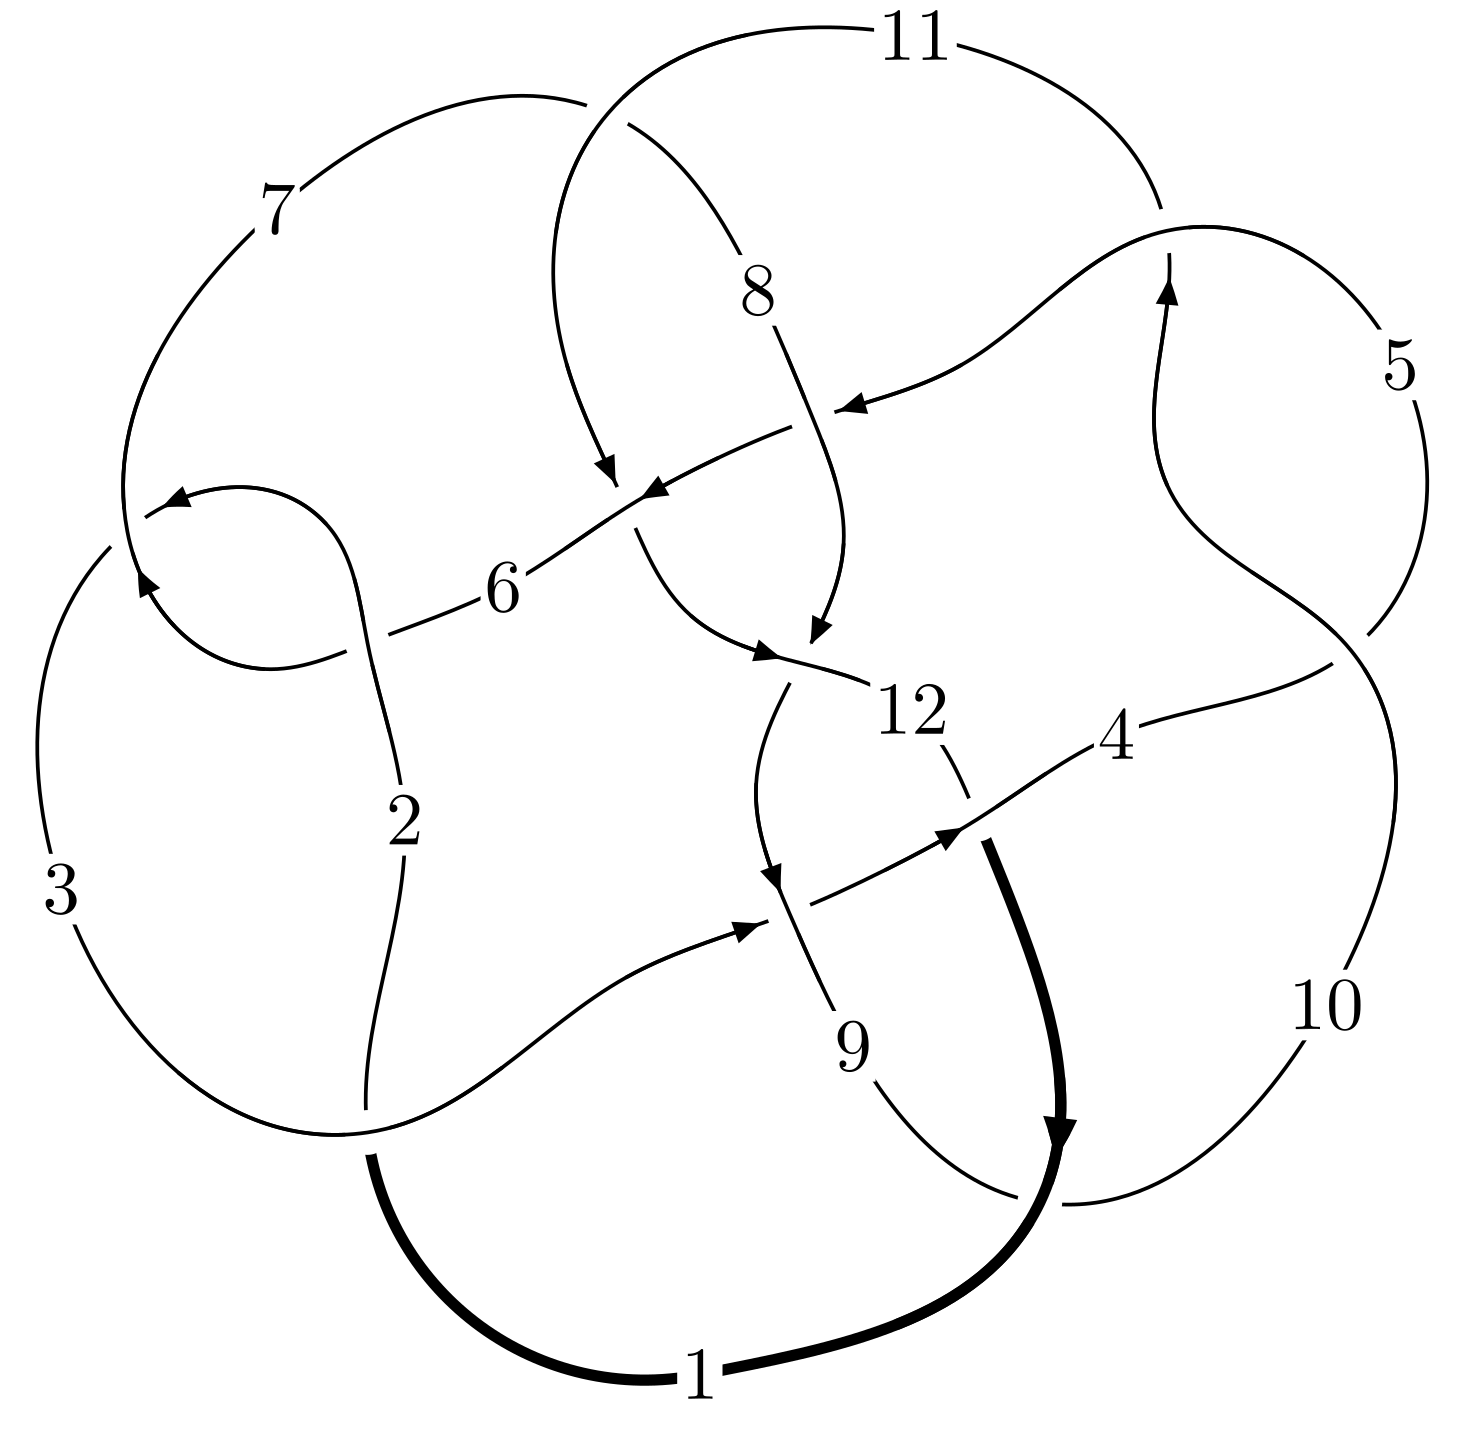
\includegraphics[width=112pt]{../../../GIT/diagram.site/Diagrams/png/1368_12a_0567.png}\\
\ \ \ A knot diagram\footnotemark}&
\allowdisplaybreaks
\textbf{Linearized knot diagam} \\
\cline{2-2}
 &
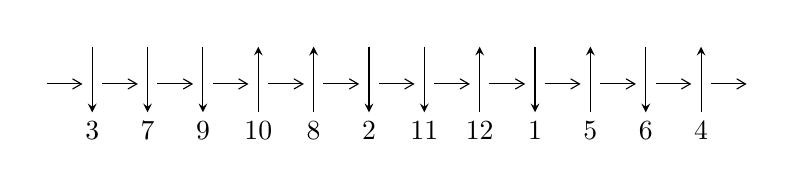
\begin{tikzpicture}[x=20pt, y=17pt]
	% nodes
	\node (C0) at (0, 0) {};
	\node (C1) at (1, 0) {};
	\node (C1U) at (1, +1) {};
	\node (C1D) at (1, -1) {3};

	\node (C2) at (2, 0) {};
	\node (C2U) at (2, +1) {};
	\node (C2D) at (2, -1) {7};

	\node (C3) at (3, 0) {};
	\node (C3U) at (3, +1) {};
	\node (C3D) at (3, -1) {9};

	\node (C4) at (4, 0) {};
	\node (C4U) at (4, +1) {};
	\node (C4D) at (4, -1) {10};

	\node (C5) at (5, 0) {};
	\node (C5U) at (5, +1) {};
	\node (C5D) at (5, -1) {8};

	\node (C6) at (6, 0) {};
	\node (C6U) at (6, +1) {};
	\node (C6D) at (6, -1) {2};

	\node (C7) at (7, 0) {};
	\node (C7U) at (7, +1) {};
	\node (C7D) at (7, -1) {11};

	\node (C8) at (8, 0) {};
	\node (C8U) at (8, +1) {};
	\node (C8D) at (8, -1) {12};

	\node (C9) at (9, 0) {};
	\node (C9U) at (9, +1) {};
	\node (C9D) at (9, -1) {1};

	\node (C10) at (10, 0) {};
	\node (C10U) at (10, +1) {};
	\node (C10D) at (10, -1) {5};

	\node (C11) at (11, 0) {};
	\node (C11U) at (11, +1) {};
	\node (C11D) at (11, -1) {6};

	\node (C12) at (12, 0) {};
	\node (C12U) at (12, +1) {};
	\node (C12D) at (12, -1) {4};
	\node (C13) at (13, 0) {};

	% arrows
	\draw[->,>={angle 60}]
	(C0) edge (C1) (C1) edge (C2) (C2) edge (C3) (C3) edge (C4) (C4) edge (C5) (C5) edge (C6) (C6) edge (C7) (C7) edge (C8) (C8) edge (C9) (C9) edge (C10) (C10) edge (C11) (C11) edge (C12) (C12) edge (C13) ;	\draw[->,>=stealth]
	(C1U) edge (C1D) (C2U) edge (C2D) (C3U) edge (C3D) (C4D) edge (C4U) (C5D) edge (C5U) (C6U) edge (C6D) (C7U) edge (C7D) (C8D) edge (C8U) (C9U) edge (C9D) (C10D) edge (C10U) (C11U) edge (C11D) (C12D) edge (C12U) ;
	\end{tikzpicture} \\
\hhline{~~} \\& 
\textbf{Solving Sequence} \\ \cline{2-2} 
 &
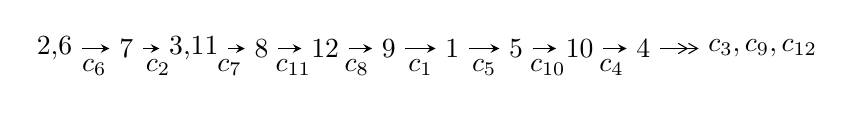
\begin{tikzpicture}[x=23pt, y=7pt]
	% node
	\node (A0) at (-1/8, 0) {2,6};
	\node (A1) at (1, 0) {7};
	\node (A2) at (33/16, 0) {3,11};
	\node (A3) at (25/8, 0) {8};
	\node (A4) at (33/8, 0) {12};
	\node (A5) at (41/8, 0) {9};
	\node (A6) at (49/8, 0) {1};
	\node (A7) at (57/8, 0) {5};
	\node (A8) at (65/8, 0) {10};
	\node (A9) at (73/8, 0) {4};
	\node (C1) at (1/2, -1) {$c_{6}$};
	\node (C2) at (3/2, -1) {$c_{2}$};
	\node (C3) at (21/8, -1) {$c_{7}$};
	\node (C4) at (29/8, -1) {$c_{11}$};
	\node (C5) at (37/8, -1) {$c_{8}$};
	\node (C6) at (45/8, -1) {$c_{1}$};
	\node (C7) at (53/8, -1) {$c_{5}$};
	\node (C8) at (61/8, -1) {$c_{10}$};
	\node (C9) at (69/8, -1) {$c_{4}$};
	\node (A10) at (11, 0) {$c_{3},c_{9},c_{12}$};

	% edge
	\draw[->,>=stealth]	
	(A0) edge (A1) (A1) edge (A2) (A2) edge (A3) (A3) edge (A4) (A4) edge (A5) (A5) edge (A6) (A6) edge (A7) (A7) edge (A8) (A8) edge (A9) ;
	\draw[->>,>={angle 60}]	
	(A9) edge (A10);
\end{tikzpicture} \\ 

\end{tabular} \\

\footnotetext{
The image of knot diagram is generated by the software ``\textbf{Draw programme}" developed by Andrew Bartholomew(\url{http://www.layer8.co.uk/maths/draw/index.htm\#Running-draw}), where we modified some parts for our purpose(\url{https://github.com/CATsTAILs/LinksPainter}).
}\phantom \\ \newline 
\centering \textbf{Ideals for irreducible components\footnotemark of $X_{\text{par}}$} 
 
\begin{align*}
I^u_{1}&=\langle 
-4.09131\times10^{58} u^{48}+1.86986\times10^{59} u^{47}+\cdots+3.40871\times10^{59} b-2.44132\times10^{59},\\
\phantom{I^u_{1}}&\phantom{= \langle  }3.95934\times10^{59} u^{48}-1.71738\times10^{60} u^{47}+\cdots+2.72697\times10^{60} a+4.13840\times10^{60},\;u^{49}-4 u^{48}+\cdots+23 u+8\rangle \\
I^u_{2}&=\langle 
5.76602\times10^{36} a u^{55}-4.95035\times10^{36} u^{55}+\cdots+4.07129\times10^{37} a-2.44952\times10^{37},\\
\phantom{I^u_{2}}&\phantom{= \langle  }-3.06643\times10^{37} a u^{55}+1.88524\times10^{37} u^{55}+\cdots-2.77446\times10^{38} a+8.18996\times10^{38},\\
\phantom{I^u_{2}}&\phantom{= \langle  }u^{56}+2 u^{55}+\cdots+6 u-1\rangle \\
I^u_{3}&=\langle 
4249 u^{14} a-18260 u^{14}+\cdots+1889 a-19853,\;391 u^{14} a-404 u^{14}+\cdots+414 a-30,\\
\phantom{I^u_{3}}&\phantom{= \langle  }u^{15}+u^{14}-4 u^{13}-6 u^{12}+5 u^{11}+11 u^{10}-5 u^9-15 u^8+12 u^6+3 u^5-4 u^4+2 u^2- u-1\rangle \\
I^u_{4}&=\langle 
b+u,\;- u^3+u^2+a+1,\;u^4- u^3+1\rangle \\
I^u_{5}&=\langle 
u^2+b-1,\;u^2+a-1,\;u^3- u+1\rangle \\
\\
\end{align*}
\raggedright * 5 irreducible components of $\dim_{\mathbb{C}}=0$, with total 198 representations.\\
\footnotetext{All coefficients of polynomials are rational numbers. But the coefficients are sometimes approximated in decimal forms when there is not enough margin.}
\newpage
\renewcommand{\arraystretch}{1}
\centering \section*{I. $I^u_{1}= \langle -4.09\times10^{58} u^{48}+1.87\times10^{59} u^{47}+\cdots+3.41\times10^{59} b-2.44\times10^{59},\;3.96\times10^{59} u^{48}-1.72\times10^{60} u^{47}+\cdots+2.73\times10^{60} a+4.14\times10^{60},\;u^{49}-4 u^{48}+\cdots+23 u+8 \rangle$}
\flushleft \textbf{(i) Arc colorings}\\
\begin{tabular}{m{7pt} m{180pt} m{7pt} m{180pt} }
\flushright $a_{2}=$&$\begin{pmatrix}0\\u\end{pmatrix}$ \\
\flushright $a_{6}=$&$\begin{pmatrix}1\\0\end{pmatrix}$ \\
\flushright $a_{7}=$&$\begin{pmatrix}1\\u^2\end{pmatrix}$ \\
\flushright $a_{3}=$&$\begin{pmatrix}- u\\- u^3+u\end{pmatrix}$ \\
\flushright $a_{11}=$&$\begin{pmatrix}-0.145192 u^{48}+0.629778 u^{47}+\cdots-4.54924 u-1.51758\\0.120025 u^{48}-0.548555 u^{47}+\cdots+0.606531 u+0.716200\end{pmatrix}$ \\
\flushright $a_{8}=$&$\begin{pmatrix}0.189703 u^{48}-0.932656 u^{47}+\cdots+2.33137 u+9.48319\\-0.186093 u^{48}+0.727299 u^{47}+\cdots+1.76881 u-1.97297\end{pmatrix}$ \\
\flushright $a_{12}=$&$\begin{pmatrix}-0.265217 u^{48}+1.17833 u^{47}+\cdots-5.15578 u-2.23378\\0.120025 u^{48}-0.548555 u^{47}+\cdots+0.606531 u+0.716200\end{pmatrix}$ \\
\flushright $a_{9}=$&$\begin{pmatrix}0.206990 u^{48}-0.945493 u^{47}+\cdots+14.0872 u+3.57428\\-0.0567147 u^{48}+0.239211 u^{47}+\cdots-2.81883 u-1.18146\end{pmatrix}$ \\
\flushright $a_{1}=$&$\begin{pmatrix}u^3\\u^5- u^3+u\end{pmatrix}$ \\
\flushright $a_{5}=$&$\begin{pmatrix}-0.562435 u^{48}+2.55775 u^{47}+\cdots-12.9670 u-8.28467\\0.114740 u^{48}-0.470163 u^{47}+\cdots+4.03582 u+2.02292\end{pmatrix}$ \\
\flushright $a_{10}=$&$\begin{pmatrix}0.169778 u^{48}-0.780402 u^{47}+\cdots+14.4821 u+3.69444\\-0.0697919 u^{48}+0.249032 u^{47}+\cdots-1.50204 u-0.424318\end{pmatrix}$ \\
\flushright $a_{4}=$&$\begin{pmatrix}-0.180310 u^{48}+0.904758 u^{47}+\cdots-9.77548 u-7.99759\\0.107011 u^{48}-0.544666 u^{47}+\cdots+2.86335 u+2.67307\end{pmatrix}$\\&\end{tabular}
\flushleft \textbf{(ii) Obstruction class $= -1$}\\~\\
\flushleft \textbf{(iii) Cusp Shapes $= -0.767693 u^{48}+3.20767 u^{47}+\cdots-21.2132 u-8.56327$}\\~\\
\newpage\renewcommand{\arraystretch}{1}
\flushleft \textbf{(iv) u-Polynomials at the component}\newline \\
\begin{tabular}{m{50pt}|m{274pt}}
Crossings & \hspace{64pt}u-Polynomials at each crossing \\
\hline $$\begin{aligned}c_{1}\end{aligned}$$&$\begin{aligned}
&u^{49}+16 u^{48}+\cdots+1553 u+64
\end{aligned}$\\
\hline $$\begin{aligned}c_{2},c_{6}\end{aligned}$$&$\begin{aligned}
&u^{49}-4 u^{48}+\cdots+23 u+8
\end{aligned}$\\
\hline $$\begin{aligned}c_{3},c_{11}\end{aligned}$$&$\begin{aligned}
&23(23 u^{49}+48 u^{48}+\cdots+4 u+1)
\end{aligned}$\\
\hline $$\begin{aligned}c_{4},c_{10}\end{aligned}$$&$\begin{aligned}
&23(23 u^{49}+117 u^{48}+\cdots-2048 u-256)
\end{aligned}$\\
\hline $$\begin{aligned}c_{5},c_{12}\end{aligned}$$&$\begin{aligned}
&u^{49}+4 u^{48}+\cdots+2 u-23
\end{aligned}$\\
\hline $$\begin{aligned}c_{7},c_{9}\end{aligned}$$&$\begin{aligned}
&u^{49}-4 u^{48}+\cdots-202 u+23
\end{aligned}$\\
\hline $$\begin{aligned}c_{8}\end{aligned}$$&$\begin{aligned}
&u^{49}-8 u^{48}+\cdots+84571 u-12398
\end{aligned}$\\
\hline
\end{tabular}\\~\\
\newpage\renewcommand{\arraystretch}{1}
\flushleft \textbf{(v) Riley Polynomials at the component}\newline \\
\begin{tabular}{m{50pt}|m{274pt}}
Crossings & \hspace{64pt}Riley Polynomials at each crossing \\
\hline $$\begin{aligned}c_{1}\end{aligned}$$&$\begin{aligned}
&y^{49}+16 y^{48}+\cdots-2527 y-4096
\end{aligned}$\\
\hline $$\begin{aligned}c_{2},c_{6}\end{aligned}$$&$\begin{aligned}
&y^{49}-16 y^{48}+\cdots+1553 y-64
\end{aligned}$\\
\hline $$\begin{aligned}c_{3},c_{11}\end{aligned}$$&$\begin{aligned}
&529(529 y^{49}-4328 y^{48}+\cdots+8 y-1)
\end{aligned}$\\
\hline $$\begin{aligned}c_{4},c_{10}\end{aligned}$$&$\begin{aligned}
&529(529 y^{49}-23901 y^{48}+\cdots-1048576 y-65536)
\end{aligned}$\\
\hline $$\begin{aligned}c_{5},c_{12}\end{aligned}$$&$\begin{aligned}
&y^{49}-4 y^{48}+\cdots-2480 y-529
\end{aligned}$\\
\hline $$\begin{aligned}c_{7},c_{9}\end{aligned}$$&$\begin{aligned}
&y^{49}+16 y^{48}+\cdots+5108 y-529
\end{aligned}$\\
\hline $$\begin{aligned}c_{8}\end{aligned}$$&$\begin{aligned}
&y^{49}+2 y^{48}+\cdots+658603173 y-153710404
\end{aligned}$\\
\hline
\end{tabular}\\~\\
\newpage\flushleft \textbf{(vi) Complex Volumes and Cusp Shapes}
$$\begin{array}{c|c|c}  
\text{Solutions to }I^u_{1}& \I (\text{vol} + \sqrt{-1}CS) & \text{Cusp shape}\\
 \hline 
\begin{aligned}
u &= -0.990760 + 0.010241 I \\
a &= \phantom{-}1.66046 - 1.49171 I \\
b &= \phantom{-}0.575647 - 0.169924 I\end{aligned}
 & -0.30315 + 5.10924 I & -9.01712 - 6.22750 I \\ \hline\begin{aligned}
u &= -0.990760 - 0.010241 I \\
a &= \phantom{-}1.66046 + 1.49171 I \\
b &= \phantom{-}0.575647 + 0.169924 I\end{aligned}
 & -0.30315 - 5.10924 I & -9.01712 + 6.22750 I \\ \hline\begin{aligned}
u &= \phantom{-}1.012260 + 0.023476 I \\
a &= -1.68942 + 0.80249 I \\
b &= -0.727210 + 0.167304 I\end{aligned}
 & -4.31448 + 1.69841 I & -13.26922 - 4.56796 I \\ \hline\begin{aligned}
u &= \phantom{-}1.012260 - 0.023476 I \\
a &= -1.68942 - 0.80249 I \\
b &= -0.727210 - 0.167304 I\end{aligned}
 & -4.31448 - 1.69841 I & -13.26922 + 4.56796 I \\ \hline\begin{aligned}
u &= -0.312749 + 0.928676 I \\
a &= \phantom{-}0.216831 - 0.264675 I \\
b &= -0.577562 + 0.648919 I\end{aligned}
 & \phantom{-}1.60781 + 4.77505 I & \phantom{-}0.7752 - 16.7290 I \\ \hline\begin{aligned}
u &= -0.312749 - 0.928676 I \\
a &= \phantom{-}0.216831 + 0.264675 I \\
b &= -0.577562 - 0.648919 I\end{aligned}
 & \phantom{-}1.60781 - 4.77505 I & \phantom{-}0.7752 + 16.7290 I \\ \hline\begin{aligned}
u &= \phantom{-}0.853950 + 0.601895 I \\
a &= \phantom{-}0.91949 - 1.33690 I \\
b &= \phantom{-}0.603418 + 0.748102 I\end{aligned}
 & \phantom{-}3.57906 - 3.77603 I & \phantom{-}0.68519 + 6.98344 I \\ \hline\begin{aligned}
u &= \phantom{-}0.853950 - 0.601895 I \\
a &= \phantom{-}0.91949 + 1.33690 I \\
b &= \phantom{-}0.603418 - 0.748102 I\end{aligned}
 & \phantom{-}3.57906 + 3.77603 I & \phantom{-}0.68519 - 6.98344 I \\ \hline\begin{aligned}
u &= \phantom{-}0.751553 + 0.728094 I \\
a &= -1.098480 + 0.238897 I \\
b &= -0.917649 + 0.653286 I\end{aligned}
 & \phantom{-}4.63095 + 4.66427 I & -0.48019 - 6.24279 I \\ \hline\begin{aligned}
u &= \phantom{-}0.751553 - 0.728094 I \\
a &= -1.098480 - 0.238897 I \\
b &= -0.917649 - 0.653286 I\end{aligned}
 & \phantom{-}4.63095 - 4.66427 I & -0.48019 + 6.24279 I\\
 \hline 
 \end{array}$$\newpage$$\begin{array}{c|c|c}  
\text{Solutions to }I^u_{1}& \I (\text{vol} + \sqrt{-1}CS) & \text{Cusp shape}\\
 \hline 
\begin{aligned}
u &= -0.622417 + 0.699695 I \\
a &= \phantom{-}0.511387 + 0.269950 I \\
b &= \phantom{-}0.813837 + 0.666017 I\end{aligned}
 & \phantom{-}0.67081 - 2.28505 I & -5.95751 + 2.10511 I \\ \hline\begin{aligned}
u &= -0.622417 - 0.699695 I \\
a &= \phantom{-}0.511387 - 0.269950 I \\
b &= \phantom{-}0.813837 - 0.666017 I\end{aligned}
 & \phantom{-}0.67081 + 2.28505 I & -5.95751 - 2.10511 I \\ \hline\begin{aligned}
u &= -0.679488 + 0.852718 I \\
a &= \phantom{-}0.367118 - 0.009690 I \\
b &= -0.91748 - 1.39279 I\end{aligned}
 & \phantom{-}3.85833 - 8.18929 I & \phantom{-}1.17804 + 7.15730 I \\ \hline\begin{aligned}
u &= -0.679488 - 0.852718 I \\
a &= \phantom{-}0.367118 + 0.009690 I \\
b &= -0.91748 + 1.39279 I\end{aligned}
 & \phantom{-}3.85833 + 8.18929 I & \phantom{-}1.17804 - 7.15730 I \\ \hline\begin{aligned}
u &= \phantom{-}0.969892 + 0.566315 I \\
a &= \phantom{-}0.464777 - 0.615118 I \\
b &= -0.188565 + 0.396771 I\end{aligned}
 & \phantom{-}3.35118 - 0.71038 I & -1.12350 - 1.34429 I \\ \hline\begin{aligned}
u &= \phantom{-}0.969892 - 0.566315 I \\
a &= \phantom{-}0.464777 + 0.615118 I \\
b &= -0.188565 - 0.396771 I\end{aligned}
 & \phantom{-}3.35118 + 0.71038 I & -1.12350 + 1.34429 I \\ \hline\begin{aligned}
u &= \phantom{-}0.679113 + 0.905010 I \\
a &= \phantom{-}0.248678 - 0.766030 I \\
b &= \phantom{-}0.349493 - 0.169174 I\end{aligned}
 & \phantom{-}5.29678 - 4.75824 I & -1.81791 + 6.68023 I \\ \hline\begin{aligned}
u &= \phantom{-}0.679113 - 0.905010 I \\
a &= \phantom{-}0.248678 + 0.766030 I \\
b &= \phantom{-}0.349493 + 0.169174 I\end{aligned}
 & \phantom{-}5.29678 + 4.75824 I & -1.81791 - 6.68023 I \\ \hline\begin{aligned}
u &= \phantom{-}1.132310 + 0.186560 I \\
a &= \phantom{-}1.68536 + 0.59737 I \\
b &= \phantom{-}1.086950 + 0.852635 I\end{aligned}
 & -3.21951 - 7.86938 I & -6.63301 + 8.97427 I \\ \hline\begin{aligned}
u &= \phantom{-}1.132310 - 0.186560 I \\
a &= \phantom{-}1.68536 - 0.59737 I \\
b &= \phantom{-}1.086950 - 0.852635 I\end{aligned}
 & -3.21951 + 7.86938 I & -6.63301 - 8.97427 I\\
 \hline 
 \end{array}$$\newpage$$\begin{array}{c|c|c}  
\text{Solutions to }I^u_{1}& \I (\text{vol} + \sqrt{-1}CS) & \text{Cusp shape}\\
 \hline 
\begin{aligned}
u &= -0.832906\phantom{ +0.000000I} \\
a &= \phantom{-}3.68483\phantom{ +0.000000I} \\
b &= \phantom{-}2.05274\phantom{ +0.000000I}\end{aligned}
 & \phantom{-}0.673510\phantom{ +0.000000I} & -30.4930\phantom{ +0.000000I} \\ \hline\begin{aligned}
u &= -1.151700 + 0.226303 I \\
a &= \phantom{-}0.787962 + 0.316767 I \\
b &= \phantom{-}0.775756 + 0.006400 I\end{aligned}
 & -2.35055 + 0.22485 I & -5.48316 - 6.06612 I \\ \hline\begin{aligned}
u &= -1.151700 - 0.226303 I \\
a &= \phantom{-}0.787962 - 0.316767 I \\
b &= \phantom{-}0.775756 - 0.006400 I\end{aligned}
 & -2.35055 - 0.22485 I & -5.48316 + 6.06612 I \\ \hline\begin{aligned}
u &= \phantom{-}0.963159 + 0.696372 I \\
a &= \phantom{-}2.02429 - 0.69272 I \\
b &= \phantom{-}1.009660 + 0.509444 I\end{aligned}
 & \phantom{-}3.98032 - 10.12050 I & -2.53052 + 11.41214 I \\ \hline\begin{aligned}
u &= \phantom{-}0.963159 - 0.696372 I \\
a &= \phantom{-}2.02429 + 0.69272 I \\
b &= \phantom{-}1.009660 - 0.509444 I\end{aligned}
 & \phantom{-}3.98032 + 10.12050 I & -2.53052 - 11.41214 I \\ \hline\begin{aligned}
u &= -1.007620 + 0.650126 I \\
a &= -1.71961 - 0.69174 I \\
b &= -0.983070 + 0.578977 I\end{aligned}
 & -0.46730 + 7.50602 I & -10.62062 - 8.40734 I \\ \hline\begin{aligned}
u &= -1.007620 - 0.650126 I \\
a &= -1.71961 + 0.69174 I \\
b &= -0.983070 - 0.578977 I\end{aligned}
 & -0.46730 - 7.50602 I & -10.62062 + 8.40734 I \\ \hline\begin{aligned}
u &= \phantom{-}0.664979 + 1.010740 I \\
a &= \phantom{-}0.0490397 - 0.0679405 I \\
b &= \phantom{-}0.96811 - 1.21500 I\end{aligned}
 & \phantom{-}10.7432 + 14.0283 I & \phantom{-}3.41403 - 6.66068 I \\ \hline\begin{aligned}
u &= \phantom{-}0.664979 - 1.010740 I \\
a &= \phantom{-}0.0490397 + 0.0679405 I \\
b &= \phantom{-}0.96811 + 1.21500 I\end{aligned}
 & \phantom{-}10.7432 - 14.0283 I & \phantom{-}3.41403 + 6.66068 I \\ \hline\begin{aligned}
u &= -0.940771 + 0.774401 I \\
a &= -0.479255 - 0.605762 I \\
b &= -0.156878 + 0.437253 I\end{aligned}
 & \phantom{-}0.22555 + 2.99206 I & -9.23818 - 4.58020 I\\
 \hline 
 \end{array}$$\newpage$$\begin{array}{c|c|c}  
\text{Solutions to }I^u_{1}& \I (\text{vol} + \sqrt{-1}CS) & \text{Cusp shape}\\
 \hline 
\begin{aligned}
u &= -0.940771 - 0.774401 I \\
a &= -0.479255 + 0.605762 I \\
b &= -0.156878 - 0.437253 I\end{aligned}
 & \phantom{-}0.22555 - 2.99206 I & -9.23818 + 4.58020 I \\ \hline\begin{aligned}
u &= \phantom{-}0.921978 + 0.832111 I \\
a &= -0.202913 + 0.593928 I \\
b &= -1.088090 + 0.407029 I\end{aligned}
 & \phantom{-}4.88611 - 1.92773 I & -4.45196 - 2.98835 I \\ \hline\begin{aligned}
u &= \phantom{-}0.921978 - 0.832111 I \\
a &= -0.202913 - 0.593928 I \\
b &= -1.088090 - 0.407029 I\end{aligned}
 & \phantom{-}4.88611 + 1.92773 I & -4.45196 + 2.98835 I \\ \hline\begin{aligned}
u &= -1.032470 + 0.738931 I \\
a &= \phantom{-}1.81198 + 0.70417 I \\
b &= \phantom{-}1.10239 - 1.44459 I\end{aligned}
 & \phantom{-}2.7816 + 14.1245 I & \phantom{-0.000000 } 0. - 11.47530 I \\ \hline\begin{aligned}
u &= -1.032470 - 0.738931 I \\
a &= \phantom{-}1.81198 - 0.70417 I \\
b &= \phantom{-}1.10239 + 1.44459 I\end{aligned}
 & \phantom{-}2.7816 - 14.1245 I & \phantom{-0.000000 -}0. + 11.47530 I \\ \hline\begin{aligned}
u &= \phantom{-}0.945419 + 0.920642 I \\
a &= \phantom{-}0.610439 - 0.546138 I \\
b &= \phantom{-}0.717987 + 0.408108 I\end{aligned}
 & \phantom{-}4.99471 - 4.54872 I & \phantom{-0.000000 -}0. + 8.24622 I \\ \hline\begin{aligned}
u &= \phantom{-}0.945419 - 0.920642 I \\
a &= \phantom{-}0.610439 + 0.546138 I \\
b &= \phantom{-}0.717987 - 0.408108 I\end{aligned}
 & \phantom{-}4.99471 + 4.54872 I & \phantom{-0.000000 } 0. - 8.24622 I \\ \hline\begin{aligned}
u &= \phantom{-}0.110954 + 1.347940 I \\
a &= \phantom{-}0.0385506 + 0.0442015 I \\
b &= \phantom{-}0.608073 + 0.613858 I\end{aligned}
 & \phantom{-}7.12930 - 6.91949 I & \phantom{-0.000000 -}0. + 13.46028 I \\ \hline\begin{aligned}
u &= \phantom{-}0.110954 - 1.347940 I \\
a &= \phantom{-}0.0385506 - 0.0442015 I \\
b &= \phantom{-}0.608073 - 0.613858 I\end{aligned}
 & \phantom{-}7.12930 + 6.91949 I & \phantom{-0.000000 } 0. - 13.46028 I \\ \hline\begin{aligned}
u &= \phantom{-}1.105590 + 0.788327 I \\
a &= -1.72452 + 0.59522 I \\
b &= -1.08248 - 1.25928 I\end{aligned}
 & \phantom{-}9.3385 - 20.5675 I & \phantom{-0.000000 } 0\\
 \hline 
 \end{array}$$\newpage$$\begin{array}{c|c|c}  
\text{Solutions to }I^u_{1}& \I (\text{vol} + \sqrt{-1}CS) & \text{Cusp shape}\\
 \hline 
\begin{aligned}
u &= \phantom{-}1.105590 - 0.788327 I \\
a &= -1.72452 - 0.59522 I \\
b &= -1.08248 + 1.25928 I\end{aligned}
 & \phantom{-}9.3385 + 20.5675 I & \phantom{-0.000000 } 0 \\ \hline\begin{aligned}
u &= -1.342990 + 0.314986 I \\
a &= -1.355500 + 0.358423 I \\
b &= -0.981026 + 0.806984 I\end{aligned}
 & \phantom{-}1.72502 + 12.43410 I & \phantom{-0.000000 } 0 \\ \hline\begin{aligned}
u &= -1.342990 - 0.314986 I \\
a &= -1.355500 - 0.358423 I \\
b &= -0.981026 - 0.806984 I\end{aligned}
 & \phantom{-}1.72502 - 12.43410 I & \phantom{-0.000000 } 0 \\ \hline\begin{aligned}
u &= -0.323280 + 0.360692 I \\
a &= \phantom{-}0.615793 - 0.612104 I \\
b &= \phantom{-}0.182207 - 0.540934 I\end{aligned}
 & -0.355252 + 1.132390 I & -3.37752 - 6.52476 I \\ \hline\begin{aligned}
u &= -0.323280 - 0.360692 I \\
a &= \phantom{-}0.615793 + 0.612104 I \\
b &= \phantom{-}0.182207 + 0.540934 I\end{aligned}
 & -0.355252 - 1.132390 I & -3.37752 + 6.52476 I \\ \hline\begin{aligned}
u &= \phantom{-}0.390090\phantom{ +0.000000I} \\
a &= \phantom{-}0.833908\phantom{ +0.000000I} \\
b &= -0.714999\phantom{ +0.000000I}\end{aligned}
 & \phantom{-}3.47781\phantom{ +0.000000I} & -0.345410\phantom{ +0.000000I} \\ \hline\begin{aligned}
u &= -0.345538 + 0.146876 I \\
a &= \phantom{-}2.21115 - 2.51791 I \\
b &= -0.450186 + 0.783323 I\end{aligned}
 & \phantom{-}2.32562 + 5.47653 I & \phantom{-}5.17929 - 7.75033 I \\ \hline\begin{aligned}
u &= -0.345538 - 0.146876 I \\
a &= \phantom{-}2.21115 + 2.51791 I \\
b &= -0.450186 - 0.783323 I\end{aligned}
 & \phantom{-}2.32562 - 5.47653 I & \phantom{-}5.17929 + 7.75033 I \\ \hline\begin{aligned}
u &= \phantom{-}1.72004\phantom{ +0.000000I} \\
a &= -0.518361\phantom{ +0.000000I} \\
b &= -0.697464\phantom{ +0.000000I}\end{aligned}
 & \phantom{-}0.634491\phantom{ +0.000000I} & \phantom{-0.000000 } 0\\
 \hline 
 \end{array}$$\newpage\newpage\renewcommand{\arraystretch}{1}
\centering \section*{II. $I^u_{2}= \langle 5.77\times10^{36} a u^{55}-4.95\times10^{36} u^{55}+\cdots+4.07\times10^{37} a-2.45\times10^{37},\;-3.07\times10^{37} a u^{55}+1.89\times10^{37} u^{55}+\cdots-2.77\times10^{38} a+8.19\times10^{38},\;u^{56}+2 u^{55}+\cdots+6 u-1 \rangle$}
\flushleft \textbf{(i) Arc colorings}\\
\begin{tabular}{m{7pt} m{180pt} m{7pt} m{180pt} }
\flushright $a_{2}=$&$\begin{pmatrix}0\\u\end{pmatrix}$ \\
\flushright $a_{6}=$&$\begin{pmatrix}1\\0\end{pmatrix}$ \\
\flushright $a_{7}=$&$\begin{pmatrix}1\\u^2\end{pmatrix}$ \\
\flushright $a_{3}=$&$\begin{pmatrix}- u\\- u^3+u\end{pmatrix}$ \\
\flushright $a_{11}=$&$\begin{pmatrix}a\\-0.263852 a u^{55}+0.226528 u^{55}+\cdots-1.86302 a+1.12090\end{pmatrix}$ \\
\flushright $a_{8}=$&$\begin{pmatrix}-1.13311 a u^{55}+3.97767 u^{55}+\cdots-1.44837 a+3.96049\\0.346941 a u^{55}+0.263235 u^{55}+\cdots+0.0411106 a-1.88298\end{pmatrix}$ \\
\flushright $a_{12}=$&$\begin{pmatrix}0.263852 a u^{55}-0.226528 u^{55}+\cdots+2.86302 a-1.12090\\-0.263852 a u^{55}+0.226528 u^{55}+\cdots-1.86302 a+1.12090\end{pmatrix}$ \\
\flushright $a_{9}=$&$\begin{pmatrix}-1.48785 a u^{55}+3.09205 u^{55}+\cdots-1.35678 a+2.63162\\1.15377 a u^{55}+1.14886 u^{55}+\cdots-1.37061 a-0.554114\end{pmatrix}$ \\
\flushright $a_{1}=$&$\begin{pmatrix}u^3\\u^5- u^3+u\end{pmatrix}$ \\
\flushright $a_{5}=$&$\begin{pmatrix}0.142306 a u^{55}-3.09075 u^{55}+\cdots+3.95964 a-3.40186\\-0.296599 a u^{55}+0.0319163 u^{55}+\cdots-0.758939 a+0.440740\end{pmatrix}$ \\
\flushright $a_{10}=$&$\begin{pmatrix}-0.334078 a u^{55}+4.35457 u^{55}+\cdots-2.72739 a+1.39494\\-0.296599 a u^{55}+0.675780 u^{55}+\cdots-0.758939 a+2.05880\end{pmatrix}$ \\
\flushright $a_{4}=$&$\begin{pmatrix}-0.0113552 a u^{55}+0.787260 u^{55}+\cdots+2.03843 a-5.29814\\-0.166899 a u^{55}+0.565160 u^{55}+\cdots-1.50228 a+4.66470\end{pmatrix}$\\&\end{tabular}
\flushleft \textbf{(ii) Obstruction class $= -1$}\\~\\
\flushleft \textbf{(iii) Cusp Shapes $= 0.564168 u^{55}-0.320433 u^{54}+\cdots+1.27052 u-7.10051$}\\~\\
\newpage\renewcommand{\arraystretch}{1}
\flushleft \textbf{(iv) u-Polynomials at the component}\newline \\
\begin{tabular}{m{50pt}|m{274pt}}
Crossings & \hspace{64pt}u-Polynomials at each crossing \\
\hline $$\begin{aligned}c_{1}\end{aligned}$$&$\begin{aligned}
&(u^{56}+22 u^{55}+\cdots-30 u+1)^{2}
\end{aligned}$\\
\hline $$\begin{aligned}c_{2}\end{aligned}$$&$\begin{aligned}
&(u^{56}+2 u^{55}+\cdots+6 u-1)^{2}
\end{aligned}$\\
\hline $$\begin{aligned}c_{3}\end{aligned}$$&$\begin{aligned}
&u^{112}- u^{111}+\cdots-45277 u+4693
\end{aligned}$\\
\hline $$\begin{aligned}c_{4}\end{aligned}$$&$\begin{aligned}
&(u^{56}- u^{55}+\cdots+215 u-71)^{2}
\end{aligned}$\\
\hline $$\begin{aligned}c_{5}\end{aligned}$$&$\begin{aligned}
&u^{112}+11 u^{111}+\cdots+179619 u+54371
\end{aligned}$\\
\hline $$\begin{aligned}c_{6}\end{aligned}$$&$\begin{aligned}
&(u^{56}-2 u^{55}+\cdots-6 u-1)^{2}
\end{aligned}$\\
\hline $$\begin{aligned}c_{7}\end{aligned}$$&$\begin{aligned}
&u^{112}+7 u^{111}+\cdots-864296 u-57901
\end{aligned}$\\
\hline $$\begin{aligned}c_{8}\end{aligned}$$&$\begin{aligned}
&(u^{56}+9 u^{55}+\cdots+3202 u-5311)^{2}
\end{aligned}$\\
\hline $$\begin{aligned}c_{9}\end{aligned}$$&$\begin{aligned}
&- u^{112}+7 u^{111}+\cdots-864296 u+57901
\end{aligned}$\\
\hline $$\begin{aligned}c_{10}\end{aligned}$$&$\begin{aligned}
&(u^{56}+u^{55}+\cdots-215 u-71)^{2}
\end{aligned}$\\
\hline $$\begin{aligned}c_{11}\end{aligned}$$&$\begin{aligned}
&u^{112}+u^{111}+\cdots+45277 u+4693
\end{aligned}$\\
\hline $$\begin{aligned}c_{12}\end{aligned}$$&$\begin{aligned}
&u^{112}-11 u^{111}+\cdots-179619 u+54371
\end{aligned}$\\
\hline
\end{tabular}\\~\\
\newpage\renewcommand{\arraystretch}{1}
\flushleft \textbf{(v) Riley Polynomials at the component}\newline \\
\begin{tabular}{m{50pt}|m{274pt}}
Crossings & \hspace{64pt}Riley Polynomials at each crossing \\
\hline $$\begin{aligned}c_{1}\end{aligned}$$&$\begin{aligned}
&(y^{56}+34 y^{55}+\cdots+290 y+1)^{2}
\end{aligned}$\\
\hline $$\begin{aligned}c_{2},c_{6}\end{aligned}$$&$\begin{aligned}
&(y^{56}-22 y^{55}+\cdots+30 y+1)^{2}
\end{aligned}$\\
\hline $$\begin{aligned}c_{3},c_{11}\end{aligned}$$&$\begin{aligned}
&y^{112}+49 y^{111}+\cdots-2487957489 y+22024249
\end{aligned}$\\
\hline $$\begin{aligned}c_{4},c_{10}\end{aligned}$$&$\begin{aligned}
&(y^{56}-49 y^{55}+\cdots-29043 y+5041)^{2}
\end{aligned}$\\
\hline $$\begin{aligned}c_{5},c_{12}\end{aligned}$$&$\begin{aligned}
&y^{112}-55 y^{111}+\cdots-150031984807 y+2956205641
\end{aligned}$\\
\hline $$\begin{aligned}c_{7},c_{9}\end{aligned}$$&$\begin{aligned}
&y^{112}+37 y^{111}+\cdots-781066217638 y+3352525801
\end{aligned}$\\
\hline $$\begin{aligned}c_{8}\end{aligned}$$&$\begin{aligned}
&(y^{56}-49 y^{55}+\cdots-1194117192 y+28206721)^{2}
\end{aligned}$\\
\hline
\end{tabular}\\~\\
\newpage\flushleft \textbf{(vi) Complex Volumes and Cusp Shapes}
$$\begin{array}{c|c|c}  
\text{Solutions to }I^u_{2}& \I (\text{vol} + \sqrt{-1}CS) & \text{Cusp shape}\\
 \hline 
\begin{aligned}
u &= \phantom{-}0.671053 + 0.735319 I \\
a &= \phantom{-}0.034452 + 0.413041 I \\
b &= -1.00065 + 1.35060 I\end{aligned}
 & \phantom{-}8.15930 + 4.91971 I & \phantom{-}12.2797 - 8.5675 I \\ \hline\begin{aligned}
u &= \phantom{-}0.671053 + 0.735319 I \\
a &= -1.26603 + 2.27586 I \\
b &= \phantom{-}0.098678 - 0.462847 I\end{aligned}
 & \phantom{-}8.15930 + 4.91971 I & \phantom{-}12.2797 - 8.5675 I \\ \hline\begin{aligned}
u &= \phantom{-}0.671053 - 0.735319 I \\
a &= \phantom{-}0.034452 - 0.413041 I \\
b &= -1.00065 - 1.35060 I\end{aligned}
 & \phantom{-}8.15930 - 4.91971 I & \phantom{-}12.2797 + 8.5675 I \\ \hline\begin{aligned}
u &= \phantom{-}0.671053 - 0.735319 I \\
a &= -1.26603 - 2.27586 I \\
b &= \phantom{-}0.098678 + 0.462847 I\end{aligned}
 & \phantom{-}8.15930 - 4.91971 I & \phantom{-}12.2797 + 8.5675 I \\ \hline\begin{aligned}
u &= -0.655268 + 0.731518 I \\
a &= -0.398273 + 0.154608 I \\
b &= \phantom{-}0.019812 + 1.334000 I\end{aligned}
 & \phantom{-}8.20794 + 4.66184 I & \phantom{-}11.91846 - 7.01691 I \\ \hline\begin{aligned}
u &= -0.655268 + 0.731518 I \\
a &= -1.92896 - 1.98521 I \\
b &= -0.091543 + 0.686724 I\end{aligned}
 & \phantom{-}8.20794 + 4.66184 I & \phantom{-}11.91846 - 7.01691 I \\ \hline\begin{aligned}
u &= -0.655268 - 0.731518 I \\
a &= -0.398273 - 0.154608 I \\
b &= \phantom{-}0.019812 - 1.334000 I\end{aligned}
 & \phantom{-}8.20794 - 4.66184 I & \phantom{-}11.91846 + 7.01691 I \\ \hline\begin{aligned}
u &= -0.655268 - 0.731518 I \\
a &= -1.92896 + 1.98521 I \\
b &= -0.091543 - 0.686724 I\end{aligned}
 & \phantom{-}8.20794 - 4.66184 I & \phantom{-}11.91846 + 7.01691 I \\ \hline\begin{aligned}
u &= \phantom{-}1.051480 + 0.111605 I \\
a &= -0.970862 + 0.318740 I \\
b &= -0.59009 + 1.32672 I\end{aligned}
 & \phantom{-}3.39610 - 5.69525 I & \phantom{-}1.93131 + 6.67173 I \\ \hline\begin{aligned}
u &= \phantom{-}1.051480 + 0.111605 I \\
a &= \phantom{-}1.47223 + 1.23810 I \\
b &= \phantom{-}0.514661 + 0.883305 I\end{aligned}
 & \phantom{-}3.39610 - 5.69525 I & \phantom{-}1.93131 + 6.67173 I\\
 \hline 
 \end{array}$$\newpage$$\begin{array}{c|c|c}  
\text{Solutions to }I^u_{2}& \I (\text{vol} + \sqrt{-1}CS) & \text{Cusp shape}\\
 \hline 
\begin{aligned}
u &= \phantom{-}1.051480 - 0.111605 I \\
a &= -0.970862 - 0.318740 I \\
b &= -0.59009 - 1.32672 I\end{aligned}
 & \phantom{-}3.39610 + 5.69525 I & \phantom{-}1.93131 - 6.67173 I \\ \hline\begin{aligned}
u &= \phantom{-}1.051480 - 0.111605 I \\
a &= \phantom{-}1.47223 - 1.23810 I \\
b &= \phantom{-}0.514661 - 0.883305 I\end{aligned}
 & \phantom{-}3.39610 + 5.69525 I & \phantom{-}1.93131 - 6.67173 I \\ \hline\begin{aligned}
u &= \phantom{-}0.647956 + 0.835756 I \\
a &= \phantom{-}0.147561 - 0.081423 I \\
b &= -0.096629 - 0.884005 I\end{aligned}
 & \phantom{-}8.58456 - 3.25562 I & \phantom{-}9.50170 + 3.89012 I \\ \hline\begin{aligned}
u &= \phantom{-}0.647956 + 0.835756 I \\
a &= \phantom{-}1.33719 - 1.38588 I \\
b &= \phantom{-}1.29716 + 0.92050 I\end{aligned}
 & \phantom{-}8.58456 - 3.25562 I & \phantom{-}9.50170 + 3.89012 I \\ \hline\begin{aligned}
u &= \phantom{-}0.647956 - 0.835756 I \\
a &= \phantom{-}0.147561 + 0.081423 I \\
b &= -0.096629 + 0.884005 I\end{aligned}
 & \phantom{-}8.58456 + 3.25562 I & \phantom{-}9.50170 - 3.89012 I \\ \hline\begin{aligned}
u &= \phantom{-}0.647956 - 0.835756 I \\
a &= \phantom{-}1.33719 + 1.38588 I \\
b &= \phantom{-}1.29716 - 0.92050 I\end{aligned}
 & \phantom{-}8.58456 + 3.25562 I & \phantom{-}9.50170 - 3.89012 I \\ \hline\begin{aligned}
u &= \phantom{-}0.606316 + 0.870830 I \\
a &= \phantom{-}0.339911 + 0.114485 I \\
b &= -0.83087 + 1.24284 I\end{aligned}
 & \phantom{-}4.57895 + 2.01945 I & \phantom{-}5.91153 - 3.01862 I \\ \hline\begin{aligned}
u &= \phantom{-}0.606316 + 0.870830 I \\
a &= \phantom{-}0.236613 + 0.256096 I \\
b &= \phantom{-}0.084853 - 0.779988 I\end{aligned}
 & \phantom{-}4.57895 + 2.01945 I & \phantom{-}5.91153 - 3.01862 I \\ \hline\begin{aligned}
u &= \phantom{-}0.606316 - 0.870830 I \\
a &= \phantom{-}0.339911 - 0.114485 I \\
b &= -0.83087 - 1.24284 I\end{aligned}
 & \phantom{-}4.57895 - 2.01945 I & \phantom{-}5.91153 + 3.01862 I \\ \hline\begin{aligned}
u &= \phantom{-}0.606316 - 0.870830 I \\
a &= \phantom{-}0.236613 - 0.256096 I \\
b &= \phantom{-}0.084853 + 0.779988 I\end{aligned}
 & \phantom{-}4.57895 - 2.01945 I & \phantom{-}5.91153 + 3.01862 I\\
 \hline 
 \end{array}$$\newpage$$\begin{array}{c|c|c}  
\text{Solutions to }I^u_{2}& \I (\text{vol} + \sqrt{-1}CS) & \text{Cusp shape}\\
 \hline 
\begin{aligned}
u &= \phantom{-}0.843962 + 0.643797 I \\
a &= \phantom{-}1.42039 - 0.43709 I \\
b &= \phantom{-}0.169785 + 0.925363 I\end{aligned}
 & \phantom{-}3.18492 - 2.51394 I & \phantom{-}1.39602 + 4.07845 I \\ \hline\begin{aligned}
u &= \phantom{-}0.843962 + 0.643797 I \\
a &= \phantom{-}0.321321 - 0.313385 I \\
b &= -0.099338 + 1.112230 I\end{aligned}
 & \phantom{-}3.18492 - 2.51394 I & \phantom{-}1.39602 + 4.07845 I \\ \hline\begin{aligned}
u &= \phantom{-}0.843962 - 0.643797 I \\
a &= \phantom{-}1.42039 + 0.43709 I \\
b &= \phantom{-}0.169785 - 0.925363 I\end{aligned}
 & \phantom{-}3.18492 + 2.51394 I & \phantom{-}1.39602 - 4.07845 I \\ \hline\begin{aligned}
u &= \phantom{-}0.843962 - 0.643797 I \\
a &= \phantom{-}0.321321 + 0.313385 I \\
b &= -0.099338 - 1.112230 I\end{aligned}
 & \phantom{-}3.18492 + 2.51394 I & \phantom{-}1.39602 - 4.07845 I \\ \hline\begin{aligned}
u &= -0.722762 + 0.789161 I \\
a &= -0.083301 + 0.139465 I \\
b &= -0.72018 - 1.28447 I\end{aligned}
 & \phantom{-}9.49380 - 5.41487 I & \phantom{-}7.18004 + 3.12682 I \\ \hline\begin{aligned}
u &= -0.722762 + 0.789161 I \\
a &= \phantom{-}1.52309 + 1.35169 I \\
b &= \phantom{-}1.49182 - 1.13675 I\end{aligned}
 & \phantom{-}9.49380 - 5.41487 I & \phantom{-}7.18004 + 3.12682 I \\ \hline\begin{aligned}
u &= -0.722762 - 0.789161 I \\
a &= -0.083301 - 0.139465 I \\
b &= -0.72018 + 1.28447 I\end{aligned}
 & \phantom{-}9.49380 + 5.41487 I & \phantom{-}7.18004 - 3.12682 I \\ \hline\begin{aligned}
u &= -0.722762 - 0.789161 I \\
a &= \phantom{-}1.52309 - 1.35169 I \\
b &= \phantom{-}1.49182 + 1.13675 I\end{aligned}
 & \phantom{-}9.49380 + 5.41487 I & \phantom{-}7.18004 - 3.12682 I \\ \hline\begin{aligned}
u &= -0.784911 + 0.730923 I \\
a &= -0.380802 + 0.936687 I \\
b &= \phantom{-}1.01727 + 1.42356 I\end{aligned}
 & \phantom{-}7.84044 + 1.14495 I & \phantom{-}9.86468 + 0.47121 I \\ \hline\begin{aligned}
u &= -0.784911 + 0.730923 I \\
a &= -0.738756 + 0.986320 I \\
b &= -0.252150 - 0.745357 I\end{aligned}
 & \phantom{-}7.84044 + 1.14495 I & \phantom{-}9.86468 + 0.47121 I\\
 \hline 
 \end{array}$$\newpage$$\begin{array}{c|c|c}  
\text{Solutions to }I^u_{2}& \I (\text{vol} + \sqrt{-1}CS) & \text{Cusp shape}\\
 \hline 
\begin{aligned}
u &= -0.784911 - 0.730923 I \\
a &= -0.380802 - 0.936687 I \\
b &= \phantom{-}1.01727 - 1.42356 I\end{aligned}
 & \phantom{-}7.84044 - 1.14495 I & \phantom{-}9.86468 - 0.47121 I \\ \hline\begin{aligned}
u &= -0.784911 - 0.730923 I \\
a &= -0.738756 - 0.986320 I \\
b &= -0.252150 + 0.745357 I\end{aligned}
 & \phantom{-}7.84044 - 1.14495 I & \phantom{-}9.86468 - 0.47121 I \\ \hline\begin{aligned}
u &= -0.821390 + 0.697737 I \\
a &= -0.146388 + 0.503983 I \\
b &= \phantom{-}1.02303 + 1.37591 I\end{aligned}
 & \phantom{-}3.47674 - 1.58032 I & \phantom{-}2.87158 + 3.23738 I \\ \hline\begin{aligned}
u &= -0.821390 + 0.697737 I \\
a &= \phantom{-}1.44211 + 0.64984 I \\
b &= \phantom{-}0.023723 - 0.545974 I\end{aligned}
 & \phantom{-}3.47674 - 1.58032 I & \phantom{-}2.87158 + 3.23738 I \\ \hline\begin{aligned}
u &= -0.821390 - 0.697737 I \\
a &= -0.146388 - 0.503983 I \\
b &= \phantom{-}1.02303 - 1.37591 I\end{aligned}
 & \phantom{-}3.47674 + 1.58032 I & \phantom{-}2.87158 - 3.23738 I \\ \hline\begin{aligned}
u &= -0.821390 - 0.697737 I \\
a &= \phantom{-}1.44211 - 0.64984 I \\
b &= \phantom{-}0.023723 + 0.545974 I\end{aligned}
 & \phantom{-}3.47674 + 1.58032 I & \phantom{-}2.87158 - 3.23738 I \\ \hline\begin{aligned}
u &= \phantom{-}0.903982\phantom{ +0.000000I} \\
a &= -0.712165\phantom{ +0.000000I} \\
b &= -0.938052\phantom{ +0.000000I}\end{aligned}
 & \phantom{-}3.16663\phantom{ +0.000000I} & \phantom{-}2.67970\phantom{ +0.000000I} \\ \hline\begin{aligned}
u &= \phantom{-}0.903982\phantom{ +0.000000I} \\
a &= \phantom{-}1.55929\phantom{ +0.000000I} \\
b &= -0.0837679\phantom{ +0.000000I}\end{aligned}
 & \phantom{-}3.16663\phantom{ +0.000000I} & \phantom{-}2.67970\phantom{ +0.000000I} \\ \hline\begin{aligned}
u &= -1.100210 + 0.028227 I \\
a &= -1.188090 - 0.600760 I \\
b &= -0.490366 + 0.894894 I\end{aligned}
 & \phantom{-}2.64990 + 4.34352 I & \phantom{-}1.80546 - 6.02172 I \\ \hline\begin{aligned}
u &= -1.100210 + 0.028227 I \\
a &= \phantom{-}1.24614 - 1.32051 I \\
b &= \phantom{-}0.787569 - 0.692463 I\end{aligned}
 & \phantom{-}2.64990 + 4.34352 I & \phantom{-}1.80546 - 6.02172 I\\
 \hline 
 \end{array}$$\newpage$$\begin{array}{c|c|c}  
\text{Solutions to }I^u_{2}& \I (\text{vol} + \sqrt{-1}CS) & \text{Cusp shape}\\
 \hline 
\begin{aligned}
u &= -1.100210 - 0.028227 I \\
a &= -1.188090 + 0.600760 I \\
b &= -0.490366 - 0.894894 I\end{aligned}
 & \phantom{-}2.64990 - 4.34352 I & \phantom{-}1.80546 + 6.02172 I \\ \hline\begin{aligned}
u &= -1.100210 - 0.028227 I \\
a &= \phantom{-}1.24614 + 1.32051 I \\
b &= \phantom{-}0.787569 + 0.692463 I\end{aligned}
 & \phantom{-}2.64990 - 4.34352 I & \phantom{-}1.80546 + 6.02172 I \\ \hline\begin{aligned}
u &= \phantom{-}1.030240 + 0.406172 I \\
a &= \phantom{-}0.925326 - 0.997111 I \\
b &= \phantom{-}1.052900 - 0.017660 I\end{aligned}
 & -2.70052 - 5.63749 I & -6.44125 + 7.08904 I \\ \hline\begin{aligned}
u &= \phantom{-}1.030240 + 0.406172 I \\
a &= -2.08321 - 0.05879 I \\
b &= -0.851017 - 0.731337 I\end{aligned}
 & -2.70052 - 5.63749 I & -6.44125 + 7.08904 I \\ \hline\begin{aligned}
u &= \phantom{-}1.030240 - 0.406172 I \\
a &= \phantom{-}0.925326 + 0.997111 I \\
b &= \phantom{-}1.052900 + 0.017660 I\end{aligned}
 & -2.70052 + 5.63749 I & -6.44125 - 7.08904 I \\ \hline\begin{aligned}
u &= \phantom{-}1.030240 - 0.406172 I \\
a &= -2.08321 + 0.05879 I \\
b &= -0.851017 + 0.731337 I\end{aligned}
 & -2.70052 + 5.63749 I & -6.44125 - 7.08904 I \\ \hline\begin{aligned}
u &= \phantom{-}0.868540 + 0.705776 I \\
a &= -0.873366 - 0.293042 I \\
b &= \phantom{-}0.77653 - 1.89663 I\end{aligned}
 & \phantom{-}3.08142 - 2.70536 I & \phantom{-}1.25594 + 2.81571 I \\ \hline\begin{aligned}
u &= \phantom{-}0.868540 + 0.705776 I \\
a &= -2.11391 + 0.91929 I \\
b &= -0.94598 - 1.72806 I\end{aligned}
 & \phantom{-}3.08142 - 2.70536 I & \phantom{-}1.25594 + 2.81571 I \\ \hline\begin{aligned}
u &= \phantom{-}0.868540 - 0.705776 I \\
a &= -0.873366 + 0.293042 I \\
b &= \phantom{-}0.77653 + 1.89663 I\end{aligned}
 & \phantom{-}3.08142 + 2.70536 I & \phantom{-}1.25594 - 2.81571 I \\ \hline\begin{aligned}
u &= \phantom{-}0.868540 - 0.705776 I \\
a &= -2.11391 - 0.91929 I \\
b &= -0.94598 + 1.72806 I\end{aligned}
 & \phantom{-}3.08142 + 2.70536 I & \phantom{-}1.25594 - 2.81571 I\\
 \hline 
 \end{array}$$\newpage$$\begin{array}{c|c|c}  
\text{Solutions to }I^u_{2}& \I (\text{vol} + \sqrt{-1}CS) & \text{Cusp shape}\\
 \hline 
\begin{aligned}
u &= -1.093610 + 0.277348 I \\
a &= -0.659902 - 0.916771 I \\
b &= -0.486269 - 0.225346 I\end{aligned}
 & -3.46638 + 1.04104 I & -9.55039 - 2.30638 I \\ \hline\begin{aligned}
u &= -1.093610 + 0.277348 I \\
a &= \phantom{-}1.75845 - 0.05068 I \\
b &= \phantom{-}1.194510 - 0.627546 I\end{aligned}
 & -3.46638 + 1.04104 I & -9.55039 - 2.30638 I \\ \hline\begin{aligned}
u &= -1.093610 - 0.277348 I \\
a &= -0.659902 + 0.916771 I \\
b &= -0.486269 + 0.225346 I\end{aligned}
 & -3.46638 - 1.04104 I & -9.55039 + 2.30638 I \\ \hline\begin{aligned}
u &= -1.093610 - 0.277348 I \\
a &= \phantom{-}1.75845 + 0.05068 I \\
b &= \phantom{-}1.194510 + 0.627546 I\end{aligned}
 & -3.46638 - 1.04104 I & -9.55039 + 2.30638 I \\ \hline\begin{aligned}
u &= -0.899333 + 0.691537 I \\
a &= -0.203718 + 0.844361 I \\
b &= \phantom{-}0.056866 - 0.757996 I\end{aligned}
 & \phantom{-}3.23931 + 6.92218 I & \phantom{-}2.18653 - 9.52211 I \\ \hline\begin{aligned}
u &= -0.899333 + 0.691537 I \\
a &= -2.03977 - 0.90936 I \\
b &= -1.26485 + 1.23057 I\end{aligned}
 & \phantom{-}3.23931 + 6.92218 I & \phantom{-}2.18653 - 9.52211 I \\ \hline\begin{aligned}
u &= -0.899333 - 0.691537 I \\
a &= -0.203718 - 0.844361 I \\
b &= \phantom{-}0.056866 + 0.757996 I\end{aligned}
 & \phantom{-}3.23931 - 6.92218 I & \phantom{-}2.18653 + 9.52211 I \\ \hline\begin{aligned}
u &= -0.899333 - 0.691537 I \\
a &= -2.03977 + 0.90936 I \\
b &= -1.26485 - 1.23057 I\end{aligned}
 & \phantom{-}3.23931 - 6.92218 I & \phantom{-}2.18653 + 9.52211 I \\ \hline\begin{aligned}
u &= -0.940088 + 0.704068 I \\
a &= -1.70035 - 0.54160 I \\
b &= -1.29908 + 1.26359 I\end{aligned}
 & \phantom{-}7.36120 + 4.33888 I & \phantom{-}9.15448 - 6.40900 I \\ \hline\begin{aligned}
u &= -0.940088 + 0.704068 I \\
a &= \phantom{-}1.91123 + 0.95452 I \\
b &= \phantom{-}0.318523 - 0.620422 I\end{aligned}
 & \phantom{-}7.36120 + 4.33888 I & \phantom{-}9.15448 - 6.40900 I\\
 \hline 
 \end{array}$$\newpage$$\begin{array}{c|c|c}  
\text{Solutions to }I^u_{2}& \I (\text{vol} + \sqrt{-1}CS) & \text{Cusp shape}\\
 \hline 
\begin{aligned}
u &= -0.940088 - 0.704068 I \\
a &= -1.70035 + 0.54160 I \\
b &= -1.29908 - 1.26359 I\end{aligned}
 & \phantom{-}7.36120 - 4.33888 I & \phantom{-}9.15448 + 6.40900 I \\ \hline\begin{aligned}
u &= -0.940088 - 0.704068 I \\
a &= \phantom{-}1.91123 - 0.95452 I \\
b &= \phantom{-}0.318523 + 0.620422 I\end{aligned}
 & \phantom{-}7.36120 - 4.33888 I & \phantom{-}9.15448 + 6.40900 I \\ \hline\begin{aligned}
u &= \phantom{-}1.005220 + 0.687044 I \\
a &= -0.00656 + 1.67607 I \\
b &= -0.054365 - 0.639241 I\end{aligned}
 & \phantom{-}7.15644 - 10.37530 I & \phantom{-}10.9783 + 11.7769 I \\ \hline\begin{aligned}
u &= \phantom{-}1.005220 + 0.687044 I \\
a &= \phantom{-}2.09773 - 0.58903 I \\
b &= \phantom{-}1.22251 + 1.21995 I\end{aligned}
 & \phantom{-}7.15644 - 10.37530 I & \phantom{-}10.9783 + 11.7769 I \\ \hline\begin{aligned}
u &= \phantom{-}1.005220 - 0.687044 I \\
a &= -0.00656 - 1.67607 I \\
b &= -0.054365 + 0.639241 I\end{aligned}
 & \phantom{-}7.15644 + 10.37530 I & \phantom{-}10.9783 - 11.7769 I \\ \hline\begin{aligned}
u &= \phantom{-}1.005220 - 0.687044 I \\
a &= \phantom{-}2.09773 + 0.58903 I \\
b &= \phantom{-}1.22251 - 1.21995 I\end{aligned}
 & \phantom{-}7.15644 + 10.37530 I & \phantom{-}10.9783 - 11.7769 I \\ \hline\begin{aligned}
u &= -0.992808 + 0.724667 I \\
a &= \phantom{-}0.019537 - 1.057320 I \\
b &= -1.46147 - 1.42377 I\end{aligned}
 & \phantom{-}8.67176 + 11.13480 I & \phantom{-0.000000 } 0 \\ \hline\begin{aligned}
u &= -0.992808 + 0.724667 I \\
a &= \phantom{-}1.98474 + 0.67247 I \\
b &= \phantom{-}0.83751 - 1.21893 I\end{aligned}
 & \phantom{-}8.67176 + 11.13480 I & \phantom{-0.000000 } 0 \\ \hline\begin{aligned}
u &= -0.992808 - 0.724667 I \\
a &= \phantom{-}0.019537 + 1.057320 I \\
b &= -1.46147 + 1.42377 I\end{aligned}
 & \phantom{-}8.67176 - 11.13480 I & \phantom{-0.000000 } 0 \\ \hline\begin{aligned}
u &= -0.992808 - 0.724667 I \\
a &= \phantom{-}1.98474 - 0.67247 I \\
b &= \phantom{-}0.83751 + 1.21893 I\end{aligned}
 & \phantom{-}8.67176 - 11.13480 I & \phantom{-0.000000 } 0\\
 \hline 
 \end{array}$$\newpage$$\begin{array}{c|c|c}  
\text{Solutions to }I^u_{2}& \I (\text{vol} + \sqrt{-1}CS) & \text{Cusp shape}\\
 \hline 
\begin{aligned}
u &= \phantom{-}0.762619 + 0.091383 I \\
a &= \phantom{-}1.120040 + 0.658603 I \\
b &= \phantom{-}0.548557 - 0.901107 I\end{aligned}
 & -0.27517 + 3.46206 I & -4.92312 - 5.23114 I \\ \hline\begin{aligned}
u &= \phantom{-}0.762619 + 0.091383 I \\
a &= -1.45977 + 2.26715 I \\
b &= -1.009500 + 0.467491 I\end{aligned}
 & -0.27517 + 3.46206 I & -4.92312 - 5.23114 I \\ \hline\begin{aligned}
u &= \phantom{-}0.762619 - 0.091383 I \\
a &= \phantom{-}1.120040 - 0.658603 I \\
b &= \phantom{-}0.548557 + 0.901107 I\end{aligned}
 & -0.27517 - 3.46206 I & -4.92312 + 5.23114 I \\ \hline\begin{aligned}
u &= \phantom{-}0.762619 - 0.091383 I \\
a &= -1.45977 - 2.26715 I \\
b &= -1.009500 - 0.467491 I\end{aligned}
 & -0.27517 - 3.46206 I & -4.92312 + 5.23114 I \\ \hline\begin{aligned}
u &= -1.030070 + 0.692608 I \\
a &= \phantom{-}0.240072 - 0.874574 I \\
b &= \phantom{-}0.267916 + 0.932851 I\end{aligned}
 & \phantom{-}7.07940 + 0.81663 I & \phantom{-0.000000 } 0 \\ \hline\begin{aligned}
u &= -1.030070 + 0.692608 I \\
a &= -1.170500 + 0.289772 I \\
b &= -0.317845 + 1.099280 I\end{aligned}
 & \phantom{-}7.07940 + 0.81663 I & \phantom{-0.000000 } 0 \\ \hline\begin{aligned}
u &= -1.030070 - 0.692608 I \\
a &= \phantom{-}0.240072 + 0.874574 I \\
b &= \phantom{-}0.267916 - 0.932851 I\end{aligned}
 & \phantom{-}7.07940 - 0.81663 I & \phantom{-0.000000 } 0 \\ \hline\begin{aligned}
u &= -1.030070 - 0.692608 I \\
a &= -1.170500 - 0.289772 I \\
b &= -0.317845 - 1.099280 I\end{aligned}
 & \phantom{-}7.07940 - 0.81663 I & \phantom{-0.000000 } 0 \\ \hline\begin{aligned}
u &= -0.731482 + 0.085796 I \\
a &= \phantom{-}0.16955 - 1.56338 I \\
b &= \phantom{-}0.06539 - 1.55390 I\end{aligned}
 & -0.305860 + 0.273475 I & -5.19778 - 4.40178 I \\ \hline\begin{aligned}
u &= -0.731482 + 0.085796 I \\
a &= -1.36935 - 2.60328 I \\
b &= -0.635165 - 1.033230 I\end{aligned}
 & -0.305860 + 0.273475 I & -5.19778 - 4.40178 I\\
 \hline 
 \end{array}$$\newpage$$\begin{array}{c|c|c}  
\text{Solutions to }I^u_{2}& \I (\text{vol} + \sqrt{-1}CS) & \text{Cusp shape}\\
 \hline 
\begin{aligned}
u &= -0.731482 - 0.085796 I \\
a &= \phantom{-}0.16955 + 1.56338 I \\
b &= \phantom{-}0.06539 + 1.55390 I\end{aligned}
 & -0.305860 - 0.273475 I & -5.19778 + 4.40178 I \\ \hline\begin{aligned}
u &= -0.731482 - 0.085796 I \\
a &= -1.36935 + 2.60328 I \\
b &= -0.635165 + 1.033230 I\end{aligned}
 & -0.305860 - 0.273475 I & -5.19778 + 4.40178 I \\ \hline\begin{aligned}
u &= \phantom{-}1.060640 + 0.726908 I \\
a &= -1.146400 + 0.244174 I \\
b &= -0.281316 - 0.753506 I\end{aligned}
 & \phantom{-}3.22224 - 7.94380 I & \phantom{-0.000000 } 0 \\ \hline\begin{aligned}
u &= \phantom{-}1.060640 + 0.726908 I \\
a &= \phantom{-}1.67828 - 0.54490 I \\
b &= \phantom{-}1.10619 + 1.31938 I\end{aligned}
 & \phantom{-}3.22224 - 7.94380 I & \phantom{-0.000000 } 0 \\ \hline\begin{aligned}
u &= \phantom{-}1.060640 - 0.726908 I \\
a &= -1.146400 - 0.244174 I \\
b &= -0.281316 + 0.753506 I\end{aligned}
 & \phantom{-}3.22224 + 7.94380 I & \phantom{-0.000000 } 0 \\ \hline\begin{aligned}
u &= \phantom{-}1.060640 - 0.726908 I \\
a &= \phantom{-}1.67828 + 0.54490 I \\
b &= \phantom{-}1.10619 - 1.31938 I\end{aligned}
 & \phantom{-}3.22224 + 7.94380 I & \phantom{-0.000000 } 0 \\ \hline\begin{aligned}
u &= \phantom{-}1.060780 + 0.746153 I \\
a &= -0.868087 - 0.231573 I \\
b &= -0.098811 - 0.632183 I\end{aligned}
 & \phantom{-}7.35144 - 2.67401 I & \phantom{-0.000000 } 0 \\ \hline\begin{aligned}
u &= \phantom{-}1.060780 + 0.746153 I \\
a &= -0.171399 + 0.728699 I \\
b &= -1.29309 + 1.25741 I\end{aligned}
 & \phantom{-}7.35144 - 2.67401 I & \phantom{-0.000000 } 0 \\ \hline\begin{aligned}
u &= \phantom{-}1.060780 - 0.746153 I \\
a &= -0.868087 + 0.231573 I \\
b &= -0.098811 + 0.632183 I\end{aligned}
 & \phantom{-}7.35144 + 2.67401 I & \phantom{-0.000000 } 0 \\ \hline\begin{aligned}
u &= \phantom{-}1.060780 - 0.746153 I \\
a &= -0.171399 - 0.728699 I \\
b &= -1.29309 - 1.25741 I\end{aligned}
 & \phantom{-}7.35144 + 2.67401 I & \phantom{-0.000000 } 0\\
 \hline 
 \end{array}$$\newpage$$\begin{array}{c|c|c}  
\text{Solutions to }I^u_{2}& \I (\text{vol} + \sqrt{-1}CS) & \text{Cusp shape}\\
 \hline 
\begin{aligned}
u &= -0.639664 + 1.142700 I \\
a &= \phantom{-}0.0907454 + 0.0137080 I \\
b &= \phantom{-}0.92323 + 1.10207 I\end{aligned}
 & \phantom{-}9.64435 - 4.35767 I & \phantom{-0.000000 } 0 \\ \hline\begin{aligned}
u &= -0.639664 + 1.142700 I \\
a &= \phantom{-}0.0579156 - 0.0509173 I \\
b &= -0.004300 - 0.805991 I\end{aligned}
 & \phantom{-}9.64435 - 4.35767 I & \phantom{-0.000000 } 0 \\ \hline\begin{aligned}
u &= -0.639664 - 1.142700 I \\
a &= \phantom{-}0.0907454 - 0.0137080 I \\
b &= \phantom{-}0.92323 - 1.10207 I\end{aligned}
 & \phantom{-}9.64435 + 4.35767 I & \phantom{-0.000000 } 0 \\ \hline\begin{aligned}
u &= -0.639664 - 1.142700 I \\
a &= \phantom{-}0.0579156 + 0.0509173 I \\
b &= -0.004300 + 0.805991 I\end{aligned}
 & \phantom{-}9.64435 + 4.35767 I & \phantom{-0.000000 } 0 \\ \hline\begin{aligned}
u &= -1.39465\phantom{ +0.000000I} \\
a &= \phantom{-}0.978333\phantom{ +0.000000I} \\
b &= \phantom{-}1.15590\phantom{ +0.000000I}\end{aligned}
 & -2.62295\phantom{ +0.000000I} & \phantom{-0.000000 } 0 \\ \hline\begin{aligned}
u &= -1.39465\phantom{ +0.000000I} \\
a &= \phantom{-}0.0832108\phantom{ +0.000000I} \\
b &= \phantom{-}0.224734\phantom{ +0.000000I}\end{aligned}
 & -2.62295\phantom{ +0.000000I} & \phantom{-0.000000 } 0 \\ \hline\begin{aligned}
u &= \phantom{-}0.063466 + 0.584300 I \\
a &= \phantom{-}0.651341 + 0.089844 I \\
b &= -0.763936 - 0.319395 I\end{aligned}
 & -0.10326 + 2.06981 I & -2.12397 - 3.13917 I \\ \hline\begin{aligned}
u &= \phantom{-}0.063466 + 0.584300 I \\
a &= \phantom{-}0.298658 - 0.272978 I \\
b &= \phantom{-}0.487593 - 0.746997 I\end{aligned}
 & -0.10326 + 2.06981 I & -2.12397 - 3.13917 I \\ \hline\begin{aligned}
u &= \phantom{-}0.063466 - 0.584300 I \\
a &= \phantom{-}0.651341 - 0.089844 I \\
b &= -0.763936 + 0.319395 I\end{aligned}
 & -0.10326 - 2.06981 I & -2.12397 + 3.13917 I \\ \hline\begin{aligned}
u &= \phantom{-}0.063466 - 0.584300 I \\
a &= \phantom{-}0.298658 + 0.272978 I \\
b &= \phantom{-}0.487593 + 0.746997 I\end{aligned}
 & -0.10326 - 2.06981 I & -2.12397 + 3.13917 I\\
 \hline 
 \end{array}$$\newpage$$\begin{array}{c|c|c}  
\text{Solutions to }I^u_{2}& \I (\text{vol} + \sqrt{-1}CS) & \text{Cusp shape}\\
 \hline 
\begin{aligned}
u &= -1.15196 + 0.83596 I \\
a &= \phantom{-}0.804054 - 0.064713 I \\
b &= \phantom{-}0.275082 - 0.834297 I\end{aligned}
 & \phantom{-}8.00849 + 11.38970 I & \phantom{-0.000000 } 0 \\ \hline\begin{aligned}
u &= -1.15196 + 0.83596 I \\
a &= -1.54003 - 0.57492 I \\
b &= -1.01892 + 1.19474 I\end{aligned}
 & \phantom{-}8.00849 + 11.38970 I & \phantom{-0.000000 } 0 \\ \hline\begin{aligned}
u &= -1.15196 - 0.83596 I \\
a &= \phantom{-}0.804054 + 0.064713 I \\
b &= \phantom{-}0.275082 + 0.834297 I\end{aligned}
 & \phantom{-}8.00849 - 11.38970 I & \phantom{-0.000000 } 0 \\ \hline\begin{aligned}
u &= -1.15196 - 0.83596 I \\
a &= -1.54003 + 0.57492 I \\
b &= -1.01892 - 1.19474 I\end{aligned}
 & \phantom{-}8.00849 - 11.38970 I & \phantom{-0.000000 } 0 \\ \hline\begin{aligned}
u &= \phantom{-}0.463532\phantom{ +0.000000I} \\
a &= \phantom{-}2.74448 + 0.43284 I \\
b &= \phantom{-}0.135146 - 1.050140 I\end{aligned}
 & \phantom{-}4.83953\phantom{ +0.000000I} & \phantom{-}4.50770\phantom{ +0.000000I} \\ \hline\begin{aligned}
u &= \phantom{-}0.463532\phantom{ +0.000000I} \\
a &= \phantom{-}2.74448 - 0.43284 I \\
b &= \phantom{-}0.135146 + 1.050140 I\end{aligned}
 & \phantom{-}4.83953\phantom{ +0.000000I} & \phantom{-}4.50770\phantom{ +0.000000I} \\ \hline\begin{aligned}
u &= \phantom{-}1.67030\phantom{ +0.000000I} \\
a &= -0.563240 + 0.165349 I \\
b &= -0.714634 + 0.222707 I\end{aligned}
 & \phantom{-}0.625659\phantom{ +0.000000I} & \phantom{-0.000000 } 0 \\ \hline\begin{aligned}
u &= \phantom{-}1.67030\phantom{ +0.000000I} \\
a &= -0.563240 - 0.165349 I \\
b &= -0.714634 - 0.222707 I\end{aligned}
 & \phantom{-}0.625659\phantom{ +0.000000I} & \phantom{-0.000000 } 0 \\ \hline\begin{aligned}
u &= \phantom{-}0.069713 + 0.153745 I \\
a &= \phantom{-}1.71682 - 1.09990 I \\
b &= -0.469761 + 1.259310 I\end{aligned}
 & \phantom{-}6.94046 + 4.65477 I & -8.88344 + 1.97207 I \\ \hline\begin{aligned}
u &= \phantom{-}0.069713 + 0.153745 I \\
a &= \phantom{-}17.3267 + 5.1539 I \\
b &= \phantom{-}0.665925 + 0.156361 I\end{aligned}
 & \phantom{-}6.94046 + 4.65477 I & -8.88344 + 1.97207 I\\
 \hline 
 \end{array}$$\newpage$$\begin{array}{c|c|c}  
\text{Solutions to }I^u_{2}& \I (\text{vol} + \sqrt{-1}CS) & \text{Cusp shape}\\
 \hline 
\begin{aligned}
u &= \phantom{-}0.069713 - 0.153745 I \\
a &= \phantom{-}1.71682 + 1.09990 I \\
b &= -0.469761 - 1.259310 I\end{aligned}
 & \phantom{-}6.94046 - 4.65477 I & -8.88344 - 1.97207 I \\ \hline\begin{aligned}
u &= \phantom{-}0.069713 - 0.153745 I \\
a &= \phantom{-}17.3267 - 5.1539 I \\
b &= \phantom{-}0.665925 - 0.156361 I\end{aligned}
 & \phantom{-}6.94046 - 4.65477 I & -8.88344 - 1.97207 I\\
 \hline 
 \end{array}$$\newpage\newpage\renewcommand{\arraystretch}{1}
\centering \section*{III. $I^u_{3}= \langle 4249 u^{14} a-18260 u^{14}+\cdots+1889 a-19853,\;391 u^{14} a-404 u^{14}+\cdots+414 a-30,\;u^{15}+u^{14}+\cdots- u-1 \rangle$}
\flushleft \textbf{(i) Arc colorings}\\
\begin{tabular}{m{7pt} m{180pt} m{7pt} m{180pt} }
\flushright $a_{2}=$&$\begin{pmatrix}0\\u\end{pmatrix}$ \\
\flushright $a_{6}=$&$\begin{pmatrix}1\\0\end{pmatrix}$ \\
\flushright $a_{7}=$&$\begin{pmatrix}1\\u^2\end{pmatrix}$ \\
\flushright $a_{3}=$&$\begin{pmatrix}- u\\- u^3+u\end{pmatrix}$ \\
\flushright $a_{11}=$&$\begin{pmatrix}a\\-2.10659 a u^{14}+9.05305 u^{14}+\cdots-0.936539 a+9.84284\end{pmatrix}$ \\
\flushright $a_{8}=$&$\begin{pmatrix}4.94695 a u^{14}-1.61081 u^{14}+\cdots+7.15716 a-4.06891\\6.48438 a u^{14}-4.34804 u^{14}+\cdots+7.09767 a-6.10907\end{pmatrix}$ \\
\flushright $a_{12}=$&$\begin{pmatrix}2.10659 a u^{14}-9.05305 u^{14}+\cdots+1.93654 a-9.84284\\-2.10659 a u^{14}+9.05305 u^{14}+\cdots-0.936539 a+9.84284\end{pmatrix}$ \\
\flushright $a_{9}=$&$\begin{pmatrix}2.14031 a u^{14}+1.26971 u^{14}+\cdots+4.99554 a+0.471988\\1.29103 a u^{14}-7.22856 u^{14}+\cdots+1.25930 a-10.6500\end{pmatrix}$ \\
\flushright $a_{1}=$&$\begin{pmatrix}u^3\\u^5- u^3+u\end{pmatrix}$ \\
\flushright $a_{5}=$&$\begin{pmatrix}15.3733 a u^{14}-27.8230 u^{14}+\cdots+16.9033 a-29.4403\\2.33961 a u^{14}+2.85424 u^{14}+\cdots+2.84432 a+2.24492\end{pmatrix}$ \\
\flushright $a_{10}=$&$\begin{pmatrix}3.43133 a u^{14}+6.04115 u^{14}+\cdots+6.25483 a+3.82201\\2.33961 a u^{14}-3.14576 u^{14}+\cdots+2.84432 a-5.75508\end{pmatrix}$ \\
\flushright $a_{4}=$&$\begin{pmatrix}7.86019 a u^{14}-1.50089 u^{14}+\cdots+8.25533 a-3.58309\\-1.18542 a u^{14}+9.85527 u^{14}+\cdots-0.824492 a+4.37716\end{pmatrix}$\\&\end{tabular}
\flushleft \textbf{(ii) Obstruction class $= 1$}\\~\\
\flushleft \textbf{(iii) Cusp Shapes $= -45 u^{14}-79 u^{13}+114 u^{12}+349 u^{11}+57 u^{10}-415 u^9-99 u^8+555 u^7+433 u^6-148 u^5-227 u^4-18 u^3-17 u^2-99 u-37$}\\~\\
\newpage\renewcommand{\arraystretch}{1}
\flushleft \textbf{(iv) u-Polynomials at the component}\newline \\
\begin{tabular}{m{50pt}|m{274pt}}
Crossings & \hspace{64pt}u-Polynomials at each crossing \\
\hline $$\begin{aligned}c_{1}\end{aligned}$$&$\begin{aligned}
&(u^{15}-9 u^{14}+\cdots+5 u-1)^{2}
\end{aligned}$\\
\hline $$\begin{aligned}c_{2}\end{aligned}$$&$\begin{aligned}
&(u^{15}- u^{14}+\cdots- u+1)^{2}
\end{aligned}$\\
\hline $$\begin{aligned}c_{3},c_{11}\end{aligned}$$&$\begin{aligned}
&23(23 u^{30}+147 u^{28}+\cdots+u+1)
\end{aligned}$\\
\hline $$\begin{aligned}c_{4},c_{10}\end{aligned}$$&$\begin{aligned}
&23(23 u^{30}-428 u^{28}+\cdots-56074 u^2+361)
\end{aligned}$\\
\hline $$\begin{aligned}c_{5},c_{12}\end{aligned}$$&$\begin{aligned}
&u^{30}-4 u^{29}+\cdots+115 u+23
\end{aligned}$\\
\hline $$\begin{aligned}c_{6}\end{aligned}$$&$\begin{aligned}
&(u^{15}+u^{14}+\cdots- u-1)^{2}
\end{aligned}$\\
\hline $$\begin{aligned}c_{7},c_{9}\end{aligned}$$&$\begin{aligned}
&u^{30}+2 u^{29}+\cdots+138 u-23
\end{aligned}$\\
\hline $$\begin{aligned}c_{8}\end{aligned}$$&$\begin{aligned}
&(u^{15}-8 u^{14}+\cdots-5 u-1)^{2}
\end{aligned}$\\
\hline
\end{tabular}\\~\\
\newpage\renewcommand{\arraystretch}{1}
\flushleft \textbf{(v) Riley Polynomials at the component}\newline \\
\begin{tabular}{m{50pt}|m{274pt}}
Crossings & \hspace{64pt}Riley Polynomials at each crossing \\
\hline $$\begin{aligned}c_{1}\end{aligned}$$&$\begin{aligned}
&(y^{15}-5 y^{14}+\cdots+y-1)^{2}
\end{aligned}$\\
\hline $$\begin{aligned}c_{2},c_{6}\end{aligned}$$&$\begin{aligned}
&(y^{15}-9 y^{14}+\cdots+5 y-1)^{2}
\end{aligned}$\\
\hline $$\begin{aligned}c_{3},c_{11}\end{aligned}$$&$\begin{aligned}
&529(529 y^{30}+6762 y^{29}+\cdots-45 y+1)
\end{aligned}$\\
\hline $$\begin{aligned}c_{4},c_{10}\end{aligned}$$&$\begin{aligned}
&529(23 y^{15}-428 y^{14}+\cdots-56074 y+361)^{2}
\end{aligned}$\\
\hline $$\begin{aligned}c_{5},c_{12}\end{aligned}$$&$\begin{aligned}
&y^{30}-26 y^{29}+\cdots-4347 y+529
\end{aligned}$\\
\hline $$\begin{aligned}c_{7},c_{9}\end{aligned}$$&$\begin{aligned}
&y^{30}+10 y^{29}+\cdots-2438 y+529
\end{aligned}$\\
\hline $$\begin{aligned}c_{8}\end{aligned}$$&$\begin{aligned}
&(y^{15}-12 y^{14}+\cdots+3 y-1)^{2}
\end{aligned}$\\
\hline
\end{tabular}\\~\\
\newpage\flushleft \textbf{(vi) Complex Volumes and Cusp Shapes}
$$\begin{array}{c|c|c}  
\text{Solutions to }I^u_{3}& \I (\text{vol} + \sqrt{-1}CS) & \text{Cusp shape}\\
 \hline 
\begin{aligned}
u &= -0.904032 + 0.500962 I \\
a &= \phantom{-}0.400934 + 0.876728 I \\
b &= \phantom{-}0.069706 - 1.116930 I\end{aligned}
 & \phantom{-}4.87056 + 2.00812 I & \phantom{-}5.72627 - 3.22556 I \\ \hline\begin{aligned}
u &= -0.904032 + 0.500962 I \\
a &= \phantom{-}1.77208 - 0.00014 I \\
b &= \phantom{-}0.052148 - 0.855653 I\end{aligned}
 & \phantom{-}4.87056 + 2.00812 I & \phantom{-}5.72627 - 3.22556 I \\ \hline\begin{aligned}
u &= -0.904032 - 0.500962 I \\
a &= \phantom{-}0.400934 - 0.876728 I \\
b &= \phantom{-}0.069706 + 1.116930 I\end{aligned}
 & \phantom{-}4.87056 - 2.00812 I & \phantom{-}5.72627 + 3.22556 I \\ \hline\begin{aligned}
u &= -0.904032 - 0.500962 I \\
a &= \phantom{-}1.77208 + 0.00014 I \\
b &= \phantom{-}0.052148 + 0.855653 I\end{aligned}
 & \phantom{-}4.87056 - 2.00812 I & \phantom{-}5.72627 + 3.22556 I \\ \hline\begin{aligned}
u &= -0.604563 + 0.739867 I \\
a &= \phantom{-}0.003512 - 0.169021 I \\
b &= -0.82144 - 1.27893 I\end{aligned}
 & \phantom{-}7.78409 - 4.48024 I & \phantom{-}2.51653 - 2.10573 I \\ \hline\begin{aligned}
u &= -0.604563 + 0.739867 I \\
a &= -0.38868 - 2.08222 I \\
b &= -0.441933 + 0.363599 I\end{aligned}
 & \phantom{-}7.78409 - 4.48024 I & \phantom{-}2.51653 - 2.10573 I \\ \hline\begin{aligned}
u &= -0.604563 - 0.739867 I \\
a &= \phantom{-}0.003512 + 0.169021 I \\
b &= -0.82144 + 1.27893 I\end{aligned}
 & \phantom{-}7.78409 + 4.48024 I & \phantom{-}2.51653 + 2.10573 I \\ \hline\begin{aligned}
u &= -0.604563 - 0.739867 I \\
a &= -0.38868 + 2.08222 I \\
b &= -0.441933 - 0.363599 I\end{aligned}
 & \phantom{-}7.78409 + 4.48024 I & \phantom{-}2.51653 + 2.10573 I \\ \hline\begin{aligned}
u &= \phantom{-}0.877651 + 0.004916 I \\
a &= \phantom{-}0.085115 + 0.992994 I \\
b &= -0.291346 - 0.853722 I\end{aligned}
 & \phantom{-}1.07810 - 5.33896 I & -3.04139 + 7.29844 I \\ \hline\begin{aligned}
u &= \phantom{-}0.877651 + 0.004916 I \\
a &= \phantom{-}1.79796 + 2.08916 I \\
b &= \phantom{-}0.677587 + 0.511986 I\end{aligned}
 & \phantom{-}1.07810 - 5.33896 I & -3.04139 + 7.29844 I\\
 \hline 
 \end{array}$$\newpage$$\begin{array}{c|c|c}  
\text{Solutions to }I^u_{3}& \I (\text{vol} + \sqrt{-1}CS) & \text{Cusp shape}\\
 \hline 
\begin{aligned}
u &= \phantom{-}0.877651 - 0.004916 I \\
a &= \phantom{-}0.085115 - 0.992994 I \\
b &= -0.291346 + 0.853722 I\end{aligned}
 & \phantom{-}1.07810 + 5.33896 I & -3.04139 - 7.29844 I \\ \hline\begin{aligned}
u &= \phantom{-}0.877651 - 0.004916 I \\
a &= \phantom{-}1.79796 - 2.08916 I \\
b &= \phantom{-}0.677587 - 0.511986 I\end{aligned}
 & \phantom{-}1.07810 + 5.33896 I & -3.04139 - 7.29844 I \\ \hline\begin{aligned}
u &= \phantom{-}0.924863 + 0.711903 I \\
a &= -1.153080 + 0.162248 I \\
b &= -0.662154 - 0.614581 I\end{aligned}
 & \phantom{-}6.24642 - 2.74833 I & \phantom{-}2.99946 + 3.06733 I \\ \hline\begin{aligned}
u &= \phantom{-}0.924863 + 0.711903 I \\
a &= \phantom{-}0.378437 - 0.530946 I \\
b &= \phantom{-}0.768488 - 0.833987 I\end{aligned}
 & \phantom{-}6.24642 - 2.74833 I & \phantom{-}2.99946 + 3.06733 I \\ \hline\begin{aligned}
u &= \phantom{-}0.924863 - 0.711903 I \\
a &= -1.153080 - 0.162248 I \\
b &= -0.662154 + 0.614581 I\end{aligned}
 & \phantom{-}6.24642 + 2.74833 I & \phantom{-}2.99946 - 3.06733 I \\ \hline\begin{aligned}
u &= \phantom{-}0.924863 - 0.711903 I \\
a &= \phantom{-}0.378437 + 0.530946 I \\
b &= \phantom{-}0.768488 + 0.833987 I\end{aligned}
 & \phantom{-}6.24642 + 2.74833 I & \phantom{-}2.99946 - 3.06733 I \\ \hline\begin{aligned}
u &= -1.027220 + 0.711068 I \\
a &= \phantom{-}0.082567 - 0.636128 I \\
b &= \phantom{-}0.320419 + 0.524398 I\end{aligned}
 & \phantom{-}6.56063 + 10.08130 I & -0.80300 - 5.65611 I \\ \hline\begin{aligned}
u &= -1.027220 + 0.711068 I \\
a &= \phantom{-}1.94852 + 0.58493 I \\
b &= \phantom{-}1.07611 - 1.14951 I\end{aligned}
 & \phantom{-}6.56063 + 10.08130 I & -0.80300 - 5.65611 I \\ \hline\begin{aligned}
u &= -1.027220 - 0.711068 I \\
a &= \phantom{-}0.082567 + 0.636128 I \\
b &= \phantom{-}0.320419 - 0.524398 I\end{aligned}
 & \phantom{-}6.56063 - 10.08130 I & -0.80300 + 5.65611 I \\ \hline\begin{aligned}
u &= -1.027220 - 0.711068 I \\
a &= \phantom{-}1.94852 - 0.58493 I \\
b &= \phantom{-}1.07611 + 1.14951 I\end{aligned}
 & \phantom{-}6.56063 - 10.08130 I & -0.80300 + 5.65611 I\\
 \hline 
 \end{array}$$\newpage$$\begin{array}{c|c|c}  
\text{Solutions to }I^u_{3}& \I (\text{vol} + \sqrt{-1}CS) & \text{Cusp shape}\\
 \hline 
\begin{aligned}
u &= -1.33306\phantom{ +0.000000I} \\
a &= -0.835812\phantom{ +0.000000I} \\
b &= -0.858603\phantom{ +0.000000I}\end{aligned}
 & -2.75865\phantom{ +0.000000I} & -25.0550\phantom{ +0.000000I} \\ \hline\begin{aligned}
u &= -1.33306\phantom{ +0.000000I} \\
a &= -0.647491\phantom{ +0.000000I} \\
b &= -0.647713\phantom{ +0.000000I}\end{aligned}
 & -2.75865\phantom{ +0.000000I} & -25.0550\phantom{ +0.000000I} \\ \hline\begin{aligned}
u &= \phantom{-}0.318556 + 0.568840 I \\
a &= -0.221205 - 0.008661 I \\
b &= -0.339670 - 1.161460 I\end{aligned}
 & \phantom{-}7.22377 - 4.92438 I & \phantom{-}6.89107 + 11.55615 I \\ \hline\begin{aligned}
u &= \phantom{-}0.318556 + 0.568840 I \\
a &= \phantom{-}1.50073 + 3.42899 I \\
b &= -0.522464 + 0.107351 I\end{aligned}
 & \phantom{-}7.22377 - 4.92438 I & \phantom{-}6.89107 + 11.55615 I \\ \hline\begin{aligned}
u &= \phantom{-}0.318556 - 0.568840 I \\
a &= -0.221205 + 0.008661 I \\
b &= -0.339670 + 1.161460 I\end{aligned}
 & \phantom{-}7.22377 + 4.92438 I & \phantom{-}6.89107 - 11.55615 I \\ \hline\begin{aligned}
u &= \phantom{-}0.318556 - 0.568840 I \\
a &= \phantom{-}1.50073 - 3.42899 I \\
b &= -0.522464 - 0.107351 I\end{aligned}
 & \phantom{-}7.22377 + 4.92438 I & \phantom{-}6.89107 - 11.55615 I \\ \hline\begin{aligned}
u &= -0.619936\phantom{ +0.000000I} \\
a &= \phantom{-}0.22158 + 3.24295 I \\
b &= \phantom{-}0.28092 + 1.70648 I\end{aligned}
 & \phantom{-}0.189631\phantom{ +0.000000I} & \phantom{-}9.78680\phantom{ +0.000000I} \\ \hline\begin{aligned}
u &= -0.619936\phantom{ +0.000000I} \\
a &= \phantom{-}0.22158 - 3.24295 I \\
b &= \phantom{-}0.28092 - 1.70648 I\end{aligned}
 & \phantom{-}0.189631\phantom{ +0.000000I} & \phantom{-}9.78680\phantom{ +0.000000I} \\ \hline\begin{aligned}
u &= \phantom{-}1.78249\phantom{ +0.000000I} \\
a &= \phantom{-}0.690052\phantom{ +0.000000I} \\
b &= \phantom{-}1.02052\phantom{ +0.000000I}\end{aligned}
 & \phantom{-}0.839240\phantom{ +0.000000I} & \phantom{-}24.6900\phantom{ +0.000000I} \\ \hline\begin{aligned}
u &= \phantom{-}1.78249\phantom{ +0.000000I} \\
a &= -0.0636766\phantom{ +0.000000I} \\
b &= \phantom{-}0.153043\phantom{ +0.000000I}\end{aligned}
 & \phantom{-}0.839240\phantom{ +0.000000I} & \phantom{-}24.6900\phantom{ +0.000000I}\\
 \hline 
 \end{array}$$\newpage\newpage\renewcommand{\arraystretch}{1}
\centering \section*{IV. $I^u_{4}= \langle b+u,\;- u^3+u^2+a+1,\;u^4- u^3+1 \rangle$}
\flushleft \textbf{(i) Arc colorings}\\
\begin{tabular}{m{7pt} m{180pt} m{7pt} m{180pt} }
\flushright $a_{2}=$&$\begin{pmatrix}0\\u\end{pmatrix}$ \\
\flushright $a_{6}=$&$\begin{pmatrix}1\\0\end{pmatrix}$ \\
\flushright $a_{7}=$&$\begin{pmatrix}1\\u^2\end{pmatrix}$ \\
\flushright $a_{3}=$&$\begin{pmatrix}- u\\- u^3+u\end{pmatrix}$ \\
\flushright $a_{11}=$&$\begin{pmatrix}u^3- u^2-1\\- u\end{pmatrix}$ \\
\flushright $a_{8}=$&$\begin{pmatrix}- u^2- u+1\\- u^3+u^2\end{pmatrix}$ \\
\flushright $a_{12}=$&$\begin{pmatrix}u^3- u^2+u-1\\- u\end{pmatrix}$ \\
\flushright $a_{9}=$&$\begin{pmatrix}- u^2+u\\u^2- u\end{pmatrix}$ \\
\flushright $a_{1}=$&$\begin{pmatrix}u^3\\-1\end{pmatrix}$ \\
\flushright $a_{5}=$&$\begin{pmatrix}- u^3+u^2- u\\- u^2+u\end{pmatrix}$ \\
\flushright $a_{10}=$&$\begin{pmatrix}u^3- u^2-1\\- u\end{pmatrix}$ \\
\flushright $a_{4}=$&$\begin{pmatrix}- u^3+u^2- u\\- u^2+u\end{pmatrix}$\\&\end{tabular}
\flushleft \textbf{(ii) Obstruction class $= 1$}\\~\\
\flushleft \textbf{(iii) Cusp Shapes $= u^3+6 u^2-2$}\\~\\
\newpage\renewcommand{\arraystretch}{1}
\flushleft \textbf{(iv) u-Polynomials at the component}\newline \\
\begin{tabular}{m{50pt}|m{274pt}}
Crossings & \hspace{64pt}u-Polynomials at each crossing \\
\hline $$\begin{aligned}c_{1},c_{7},c_{9}\end{aligned}$$&$\begin{aligned}
&u^4- u^3+2 u^2+1
\end{aligned}$\\
\hline $$\begin{aligned}c_{2}\end{aligned}$$&$\begin{aligned}
&u^4+u^3+1
\end{aligned}$\\
\hline $$\begin{aligned}c_{3},c_{6},c_{11}\end{aligned}$$&$\begin{aligned}
&u^4- u^3+1
\end{aligned}$\\
\hline $$\begin{aligned}c_{4},c_{10}\end{aligned}$$&$\begin{aligned}
&u^4
\end{aligned}$\\
\hline $$\begin{aligned}c_{5},c_{12}\end{aligned}$$&$\begin{aligned}
&u^4- u+1
\end{aligned}$\\
\hline $$\begin{aligned}c_{8}\end{aligned}$$&$\begin{aligned}
&u^4+3 u^3+5 u^2+5 u+3
\end{aligned}$\\
\hline
\end{tabular}\\~\\
\newpage\renewcommand{\arraystretch}{1}
\flushleft \textbf{(v) Riley Polynomials at the component}\newline \\
\begin{tabular}{m{50pt}|m{274pt}}
Crossings & \hspace{64pt}Riley Polynomials at each crossing \\
\hline $$\begin{aligned}c_{1},c_{7},c_{9}\end{aligned}$$&$\begin{aligned}
&y^4+3 y^3+6 y^2+4 y+1
\end{aligned}$\\
\hline $$\begin{aligned}c_{2},c_{3},c_{6}\\c_{11}\end{aligned}$$&$\begin{aligned}
&y^4- y^3+2 y^2+1
\end{aligned}$\\
\hline $$\begin{aligned}c_{4},c_{10}\end{aligned}$$&$\begin{aligned}
&y^4
\end{aligned}$\\
\hline $$\begin{aligned}c_{5},c_{12}\end{aligned}$$&$\begin{aligned}
&y^4+2 y^2- y+1
\end{aligned}$\\
\hline $$\begin{aligned}c_{8}\end{aligned}$$&$\begin{aligned}
&y^4+y^3+y^2+5 y+9
\end{aligned}$\\
\hline
\end{tabular}\\~\\
\newpage\flushleft \textbf{(vi) Complex Volumes and Cusp Shapes}
$$\begin{array}{c|c|c}  
\text{Solutions to }I^u_{4}& \I (\text{vol} + \sqrt{-1}CS) & \text{Cusp shape}\\
 \hline 
\begin{aligned}
u &= -0.518913 + 0.666610 I \\
a &= -0.272864 + 0.934099 I \\
b &= \phantom{-}0.518913 - 0.666610 I\end{aligned}
 & \phantom{-}1.43949 + 4.22398 I & -2.49855 - 3.90867 I \\ \hline\begin{aligned}
u &= -0.518913 - 0.666610 I \\
a &= -0.272864 - 0.934099 I \\
b &= \phantom{-}0.518913 + 0.666610 I\end{aligned}
 & \phantom{-}1.43949 - 4.22398 I & -2.49855 + 3.90867 I \\ \hline\begin{aligned}
u &= \phantom{-}1.018910 + 0.602565 I \\
a &= -1.72714 + 0.43001 I \\
b &= -1.018910 - 0.602565 I\end{aligned}
 & \phantom{-}0.20545 - 7.54387 I & \phantom{-}1.99855 + 9.02548 I \\ \hline\begin{aligned}
u &= \phantom{-}1.018910 - 0.602565 I \\
a &= -1.72714 - 0.43001 I \\
b &= -1.018910 + 0.602565 I\end{aligned}
 & \phantom{-}0.20545 + 7.54387 I & \phantom{-}1.99855 - 9.02548 I\\
 \hline 
 \end{array}$$\newpage\newpage\renewcommand{\arraystretch}{1}
\centering \section*{V. $I^u_{5}= \langle u^2+b-1,\;u^2+a-1,\;u^3- u+1 \rangle$}
\flushleft \textbf{(i) Arc colorings}\\
\begin{tabular}{m{7pt} m{180pt} m{7pt} m{180pt} }
\flushright $a_{2}=$&$\begin{pmatrix}0\\u\end{pmatrix}$ \\
\flushright $a_{6}=$&$\begin{pmatrix}1\\0\end{pmatrix}$ \\
\flushright $a_{7}=$&$\begin{pmatrix}1\\u^2\end{pmatrix}$ \\
\flushright $a_{3}=$&$\begin{pmatrix}- u\\1\end{pmatrix}$ \\
\flushright $a_{11}=$&$\begin{pmatrix}- u^2+1\\- u^2+1\end{pmatrix}$ \\
\flushright $a_{8}=$&$\begin{pmatrix}- u^2- u+1\\- u\end{pmatrix}$ \\
\flushright $a_{12}=$&$\begin{pmatrix}0\\- u^2+1\end{pmatrix}$ \\
\flushright $a_{9}=$&$\begin{pmatrix}- u^2- u+1\\1\end{pmatrix}$ \\
\flushright $a_{1}=$&$\begin{pmatrix}u-1\\- u^2+u\end{pmatrix}$ \\
\flushright $a_{5}=$&$\begin{pmatrix}u^2\\u^2\end{pmatrix}$ \\
\flushright $a_{10}=$&$\begin{pmatrix}- u^2+1\\- u^2+1\end{pmatrix}$ \\
\flushright $a_{4}=$&$\begin{pmatrix}u^2\\u^2\end{pmatrix}$\\&\end{tabular}
\flushleft \textbf{(ii) Obstruction class $= 1$}\\~\\
\flushleft \textbf{(iii) Cusp Shapes $= -11 u^2+4 u+1$}\\~\\
\newpage\renewcommand{\arraystretch}{1}
\flushleft \textbf{(iv) u-Polynomials at the component}\newline \\
\begin{tabular}{m{50pt}|m{274pt}}
Crossings & \hspace{64pt}u-Polynomials at each crossing \\
\hline $$\begin{aligned}c_{1}\end{aligned}$$&$\begin{aligned}
&u^3-2 u^2+u-1
\end{aligned}$\\
\hline $$\begin{aligned}c_{2},c_{5},c_{12}\end{aligned}$$&$\begin{aligned}
&u^3- u-1
\end{aligned}$\\
\hline $$\begin{aligned}c_{3},c_{11}\end{aligned}$$&$\begin{aligned}
&u^3+u^2-1
\end{aligned}$\\
\hline $$\begin{aligned}c_{4},c_{10}\end{aligned}$$&$\begin{aligned}
&u^3
\end{aligned}$\\
\hline $$\begin{aligned}c_{6}\end{aligned}$$&$\begin{aligned}
&u^3- u+1
\end{aligned}$\\
\hline $$\begin{aligned}c_{7},c_{9}\end{aligned}$$&$\begin{aligned}
&u^3- u^2+2 u-1
\end{aligned}$\\
\hline $$\begin{aligned}c_{8}\end{aligned}$$&$\begin{aligned}
&u^3+2 u^2+3 u+1
\end{aligned}$\\
\hline
\end{tabular}\\~\\
\newpage\renewcommand{\arraystretch}{1}
\flushleft \textbf{(v) Riley Polynomials at the component}\newline \\
\begin{tabular}{m{50pt}|m{274pt}}
Crossings & \hspace{64pt}Riley Polynomials at each crossing \\
\hline $$\begin{aligned}c_{1}\end{aligned}$$&$\begin{aligned}
&y^3-2 y^2-3 y-1
\end{aligned}$\\
\hline $$\begin{aligned}c_{2},c_{5},c_{6}\\c_{12}\end{aligned}$$&$\begin{aligned}
&y^3-2 y^2+y-1
\end{aligned}$\\
\hline $$\begin{aligned}c_{3},c_{11}\end{aligned}$$&$\begin{aligned}
&y^3- y^2+2 y-1
\end{aligned}$\\
\hline $$\begin{aligned}c_{4},c_{10}\end{aligned}$$&$\begin{aligned}
&y^3
\end{aligned}$\\
\hline $$\begin{aligned}c_{7},c_{9}\end{aligned}$$&$\begin{aligned}
&y^3+3 y^2+2 y-1
\end{aligned}$\\
\hline $$\begin{aligned}c_{8}\end{aligned}$$&$\begin{aligned}
&y^3+2 y^2+5 y-1
\end{aligned}$\\
\hline
\end{tabular}\\~\\
\newpage\flushleft \textbf{(vi) Complex Volumes and Cusp Shapes}
$$\begin{array}{c|c|c}  
\text{Solutions to }I^u_{5}& \I (\text{vol} + \sqrt{-1}CS) & \text{Cusp shape}\\
 \hline 
\begin{aligned}
u &= \phantom{-}0.662359 + 0.562280 I \\
a &= \phantom{-}0.877439 - 0.744862 I \\
b &= \phantom{-}0.877439 - 0.744862 I\end{aligned}
 & \phantom{-}1.37919 + 2.82812 I & \phantom{-}2.30126 - 5.94436 I \\ \hline\begin{aligned}
u &= \phantom{-}0.662359 - 0.562280 I \\
a &= \phantom{-}0.877439 + 0.744862 I \\
b &= \phantom{-}0.877439 + 0.744862 I\end{aligned}
 & \phantom{-}1.37919 - 2.82812 I & \phantom{-}2.30126 + 5.94436 I \\ \hline\begin{aligned}
u &= -1.32472\phantom{ +0.000000I} \\
a &= -0.754878\phantom{ +0.000000I} \\
b &= -0.754878\phantom{ +0.000000I}\end{aligned}
 & -2.75839\phantom{ +0.000000I} & -23.6030\phantom{ +0.000000I}\\
 \hline 
 \end{array}$$\newpage
\newpage\renewcommand{\arraystretch}{1}
\centering \section*{ VI. u-Polynomials}
\begin{tabular}{m{50pt}|m{274pt}}
Crossings & \hspace{64pt}u-Polynomials at each crossing \\
\hline $$\begin{aligned}c_{1}\end{aligned}$$&$\begin{aligned}
&(u^3-2 u^2+u-1)(u^4- u^3+2 u^2+1)(u^{15}-9 u^{14}+\cdots+5 u-1)^{2}\\
&\cdot(u^{49}+16 u^{48}+\cdots+1553 u+64)
\end{aligned}$\\
\hline $$\begin{aligned}c_{2}\end{aligned}$$&$\begin{aligned}
&(u^3- u-1)(u^4+u^3+1)(u^{15}- u^{14}+\cdots- u+1)^{2}\\
&\cdot(u^{49}-4 u^{48}+\cdots+23 u+8)
\end{aligned}$\\
\hline $$\begin{aligned}c_{3},c_{11}\end{aligned}$$&$\begin{aligned}
&529(u^3+u^2-1)(u^4- u^3+1)(23 u^{30}+147 u^{28}+\cdots+u+1)\\
&\cdot(23 u^{49}+48 u^{48}+\cdots+4 u+1)
\end{aligned}$\\
\hline $$\begin{aligned}c_{4},c_{10}\end{aligned}$$&$\begin{aligned}
&529u^7(23 u^{30}-428 u^{28}+\cdots-56074 u^{2}+361)\\
&\cdot(23 u^{49}+117 u^{48}+\cdots-2048 u-256)
\end{aligned}$\\
\hline $$\begin{aligned}c_{5},c_{12}\end{aligned}$$&$\begin{aligned}
&(u^3- u-1)(u^4- u+1)(u^{30}-4 u^{29}+\cdots+115 u+23)\\
&\cdot(u^{49}+4 u^{48}+\cdots+2 u-23)
\end{aligned}$\\
\hline $$\begin{aligned}c_{6}\end{aligned}$$&$\begin{aligned}
&(u^3- u+1)(u^4- u^3+1)(u^{15}+u^{14}+\cdots- u-1)^{2}\\
&\cdot(u^{49}-4 u^{48}+\cdots+23 u+8)
\end{aligned}$\\
\hline $$\begin{aligned}c_{7},c_{9}\end{aligned}$$&$\begin{aligned}
&(u^3- u^2+2 u-1)(u^4- u^3+2 u^2+1)(u^{30}+2 u^{29}+\cdots+138 u-23)\\
&\cdot(u^{49}-4 u^{48}+\cdots-202 u+23)
\end{aligned}$\\
\hline $$\begin{aligned}c_{8}\end{aligned}$$&$\begin{aligned}
&(u^3+2 u^2+3 u+1)(u^4+3 u^3+5 u^2+5 u+3)\\
&\cdot((u^{15}-8 u^{14}+\cdots-5 u-1)^{2})(u^{49}-8 u^{48}+\cdots+84571 u-12398)
\end{aligned}$\\
\hline
\end{tabular}\newpage\renewcommand{\arraystretch}{1}
\centering \section*{ VII. Riley Polynomials}
\begin{tabular}{m{50pt}|m{274pt}}
Crossings & \hspace{64pt}Riley Polynomials at each crossing \\
\hline $$\begin{aligned}c_{1}\end{aligned}$$&$\begin{aligned}
&(y^3-2 y^2-3 y-1)(y^4+3 y^3+\cdots+4 y+1)(y^{15}-5 y^{14}+\cdots+y-1)^{2}\\
&\cdot(y^{49}+16 y^{48}+\cdots-2527 y-4096)
\end{aligned}$\\
\hline $$\begin{aligned}c_{2},c_{6}\end{aligned}$$&$\begin{aligned}
&(y^3-2 y^2+y-1)(y^4- y^3+2 y^2+1)(y^{15}-9 y^{14}+\cdots+5 y-1)^{2}\\
&\cdot(y^{49}-16 y^{48}+\cdots+1553 y-64)
\end{aligned}$\\
\hline $$\begin{aligned}c_{3},c_{11}\end{aligned}$$&$\begin{aligned}
&279841(y^3- y^2+2 y-1)(y^4- y^3+2 y^2+1)\\
&\cdot(529 y^{30}+6762 y^{29}+\cdots-45 y+1)(529 y^{49}-4328 y^{48}+\cdots+8 y-1)
\end{aligned}$\\
\hline $$\begin{aligned}c_{4},c_{10}\end{aligned}$$&$\begin{aligned}
&279841y^7(23 y^{15}-428 y^{14}+\cdots-56074 y+361)^{2}\\
&\cdot(529 y^{49}-23901 y^{48}+\cdots-1048576 y-65536)
\end{aligned}$\\
\hline $$\begin{aligned}c_{5},c_{12}\end{aligned}$$&$\begin{aligned}
&(y^3-2 y^2+y-1)(y^4+2 y^2- y+1)(y^{30}-26 y^{29}+\cdots-4347 y+529)\\
&\cdot(y^{49}-4 y^{48}+\cdots-2480 y-529)
\end{aligned}$\\
\hline $$\begin{aligned}c_{7},c_{9}\end{aligned}$$&$\begin{aligned}
&(y^3+3 y^2+2 y-1)(y^4+3 y^3+6 y^2+4 y+1)\\
&\cdot(y^{30}+10 y^{29}+\cdots-2438 y+529)(y^{49}+16 y^{48}+\cdots+5108 y-529)
\end{aligned}$\\
\hline $$\begin{aligned}c_{8}\end{aligned}$$&$\begin{aligned}
&(y^3+2 y^2+5 y-1)(y^4+y^3+y^2+5 y+9)(y^{15}-12 y^{14}+\cdots+3 y-1)^{2}\\
&\cdot(y^{49}+2 y^{48}+\cdots+658603173 y-153710404)
\end{aligned}$\\
\hline
\end{tabular}
\vskip 2pc
\end{document}